\lhead{\begin{tikzpicture}[remember picture, overlay]
    \node [anchor=100,inner sep=0] (imagenIZQUIERDA) at (current page header area.north){
\includegraphics[width=18cm]{img/Encabezado.PNG}};
    \end{tikzpicture}}
    \rhead{Autor: Llamas-Nuñez}
    \rfoot{\begin{tikzpicture}[remember picture, overlay]
    \node [anchor=140,inner sep=0] (imagenDERECHA) at (current page footer area.south){
\includegraphics[width=18cm]{img/Foot.PNG}};
    \end{tikzpicture}}
    %----------------------------------------------------------------------------------------
    \lfoot{ \thepage}
    % \renewcommand{\labelenumi}{\alph{enumi}.)} 
    %----------------------------------------------------------------------------------------
    %----------------------------------------------------------------------------------------
    %	TITLE SECTION
    %----------------------------------------------------------------------------------------
    
    \setlength{\droptitle}{-5\baselineskip} % Move the title up
    \title{\textbf{ Estudio de tiempos y movimientos en el ensamble de un circuito electrónico utilizando diferentes métodos para su optimización} } % Article title
    
     \author{ 
     \textsc{Llamas Nuñez, Ana Valeria}\\ 
    %  Afiliación:
     \texttt{ Instituto Tecnológico de Querétaro } \\ 
     \texttt{Tecnológico Nacional de México  } \\ 
     \texttt{Querétaro, México}\\ 
     \texttt{ llamasnunezanavaleria@gmail.com } 
     \and 
     \textsc{Ángeles Hurtado, Luis Alberto}\\ 
    %  Afiliación:
     \texttt{ Instituto Tecnológico de Querétaro } \\ 
     \texttt{ Tecnológico Nacional de México } \\ 
     \texttt{ Querétaro, México }\\ 
     \texttt{ alb3rto.ah@gmail.com } 
    }
    
    
    %----------------------------------------------------------------------------------------
    
    % \begin{document}
    
    % Print the title
    \maketitle
    \thispagestyle{fancy}
    
    %----------------------------------------------------------------------------------------
    %	ARTICLE CONTENTS
    %----------------------------------------------------------------------------------------
    
    % \section*{Resumen}
    % \textit{Palabras clave:}
    % El resumen (ancho de página) deberá contener entre 100 y 200 palabras tipo Adobe Devangari 11 puntos.
    
    \begin{abstract}
    \noindent 
     
    
    \end{abstract}
    % 
    % 
    \textbf{\textit{Palabras clave}}: {First keyword should be the corresponding to the research area according with the authors guide. Maximum of 6 keywords.}
    % \keywords{First keyword should be the corresponding to the research area according with the authors guide. Maximum of 6 keywords.}
    
    \section{Introducción}
    
    
    % Define estudio de tiempos y movimientos
    % define que es ensamble
    % define que es circuito electronico
    % define el metodo de tiempos predeterminados
    % define optimización
    \begin{itemize}
        \item Estudio de tiempos y movimientos:
        \item Estudio
        1. m. Esfuerzo que pone el entendimiento aplicándose a conocer algo.
        2. m. Trabajo empleado en aprender y cultivar una ciencia o arte.
        \item Tiempo
        2. m. Magnitud física que permite ordenar la secuencia de los sucesos, estableciendo un pasado, un presente y un futuro, y cuya unidad en el sistema internacional es el segundo.
        \item Movimiento
        1. m. Acción y efecto de mover.
        2. m. Estado de los cuerpos mientras cambian de lugar o de posición.
        \item \textit{\textbf{ "Es una herramienta la cual implica realizar esfuerzo para aprender, comprender y mejorar la manera en que se llevan acabo las labores. En esta se analiza la secuencia de eventos que ocurren durante el trabajo realizado, empleando en este herramientas, materiales y métodos específicos."}}
        \item Ensamble:
       \textit{\textbf{ "Operación de manufactura en el cual dos o más partes separadas se unen para formar una nueva entidad " }}
       \item  Circuito electrónico 
        \item Circuito
        4. m. Recorrido previamente fijado que suele terminar en el punto de partida.
        \item Electrónico 
        6. f. Estudio y aplicación del comportamiento de los electrones en diversos medios, como el vacío, los gases y los semiconductores, sometidos a la acción de campos eléctricos y magnéticos.
        \item \textit{\textbf{" Estructura cuyo funcionamiento es crear un recorrido por el cual pueda viajar la corriente. Depende del flujo de los electrones para permitir generar, transmitir, recibir  y almacenar la información "}}
       \item  Optimización
        \textit{\textbf{1. tr. Buscar la mejor manera de realizar una actividad.}}
    
    \end{itemize}
    % 
    % 
    \section{Justificación}
    
    \begin{itemize}
        \item En base al Estudio de Trabajo durante este proyecto se busca mejorar y optimizar los tiempos y movimientos que realizara el operador buscando así mejorar la productividad, según Kanawaty en su obra «Introducción al estudio del trabajo» lo define así: "El estudio del trabajo es el examen sistemático de los métodos para realizar actividades con el fin de mejorar la utilización eficaz de los recursos y de establecer normas de rendimiento con respecto a las actividades que se están realizando". Por lo tanto este tiene como objetivo evaluar de que manera se esta llevando acabo el trabajo para así facilitar o transformar el método con el cual esta trabajando para disminuir el tiempos y movimientos innecesarios. Para así dentro de este buscar la manera mas económica y eficaz de realizar el trabajo.
        En la actualidad, se demanda una eficiencia cada vez mayor en la producción de circuitos electrónicos debido al crecimiento de la industria de la tecnología. Los fabricantes necesitan ensamblar estos circuitos de manera rápida y precisa.
        Para lograr esto, el uso de técnicas avanzadas de estudio de tiempos y movimientos durante el proceso de ensamblaje es fundamental. Se necesita una comprensión profunda de cómo se realizan las tareas y los movimientos necesarios para completar el ensamble. Esto incluye la evaluación de la eficiencia del proceso, el análisis de movimientos y el uso de tecnologías de seguimiento de tiempos.Además, se necesita una optimización continua de los métodos para reducir los tiempos de producción, minimizar los errores y mejorar la calidad del producto final.
        \item Debe de tener Referencias científicas, URL, tesis, etc.
    \end{itemize}
    % 
    % 
    \section{Descripción del problema}
    \begin{itemize}
        \item Se tiene como objetivo diseñar, mejorar e integrar sistemas productivos para ensamblar el circuito electrónico, aplicando tecnologías para su optimización. Así como desarrollar e implementar sistemas de trabajo para aumentar la productividad. Para obtener resultados concretos utilizaremos sistemas de tiempos predeterminados para establecer estándares de trabajo que promuevan la eficiencia. Para garantizar una mayor aptitud este también incluirá la realización de muestreos de trabajo para la estandarización dentro del área operativa. 
    \end{itemize}
    
    \textbf{*La incógnita científica es el elemento cuya solución incrementa el conocimiento científico.}
    % 
    % 
    \section{Fundamentación teórica}
    
    "El estudio de métodos en el registro y examen crítico sistemático de los modos de realizar actividades, con el fin de efectuar mejoras".
    Se examinaran de los métodos para realizar actividades con el fin de mejorar la utilización eficaz de los recursos y establecer normas de rendimiento con respecto a las actividades. El objetivo es evaluar la forma en que se está llevando a cabo el trabajo con el fin de facilitar o modificar el enfoque con el que está trabajando para reducir el tiempo y los movimientos innecesarios. Esto se realizara en base a los principios de la ingeniería industrial los cuales proporcionan la base para entender cómo se pueden mejorar los procesos de producción mediante el análisis, estandarización y optimización de los tiempos y movimientos.
    Se buscara establecer métodos de trabajo estándar para garantizar la uniformidad y la calidad en el proceso de ensamble. Esto implica definir pasos específicos para cada tarea, así como los tiempos y movimientos asociados a cada uno de ellos.Para ello se buscara encontrar la mejor manera de llevar a cabo el ensamble con los recursos disponibles y  así se  centrara en analizar el tiempo requerido para llevar a cabo cada una de las actividades dentro del ensamble así como los movimientos físicos que realiza el operador durante el ensamble de circuitos electrónicos. Se busca identificar movimientos innecesarios o redundantes que puedan ser eliminados o simplificados para mejorar la eficiencia.
    
    
    \begin{itemize}
        \item Se debe de retomar el tema que se planteo en la introducción, pero ahora profundizando para clarificar la incógnita científica y se pueda plantear la hipótesis.
        \item Se debe de retomar la descripción del problema, pero ahora a profundidad del (los) objeto(s) de estudio. 
        \item Se debe de profundizar en las metodologías que se ha usado para el estudio del tema.
        \item Referencias solo de artículos y libros científicos.
    \end{itemize}
    % 
    % 
    \section{Hipótesis}
    
    Es la suposición con fundamento científico relativa a la solución del problema, necesidad o de cómo se aprovecha la oportunidad con la incógnita científica y se fundamenta con: 1. Una suposición (en afirmativo o negativo) y ésta deberá vincularse con:
    2. La fundamentación científica que deberá ser precisa 3. Una entidad de comparación para probar la suposición y
    4. La variable con que se califica o cuantifica la comparación o se prueba la hipótesis.
    
    \begin{itemize}
        \item Se debe de identificar claramente la suposición científica
        \item Se debe de identificar claramente el fundamento científico
        \item Se debe identificar claramente la variable de respuesta
        \item Se debe identifican claramente las realidades o modelos contrastantes
        \item Se debe de establecer las variables asociadas, explicativas o que tienen relación funcional con la variable de respuesta
    \end{itemize}
    % 
    % 
    \section{Objetivo}
    
    \begin{itemize}
        \item Diseña, mejora e integra sistemas productivos de bienes y servicios aplicando tecnologías para su optimización
        \item Diseña, implementa y mejora sistemas de trabajo para elevar la productividad
    \end{itemize}
    
    \subsection{Objetivos específicos }
    
    \begin{itemize}
        \item Aplicar los sistemas de tiempos predeterminados como fundamento del estudio de tiempos para establecer estándares.
        \item Realizar el muestreo de trabajo para ka estandarización en el área operativa.
        
    \end{itemize}
    
    % 
    % 
    \section{Cuerpo (Metodología, modelo matemático, etc.)}
    % 
    % 
    \begin{figure}[H]
        \centering
        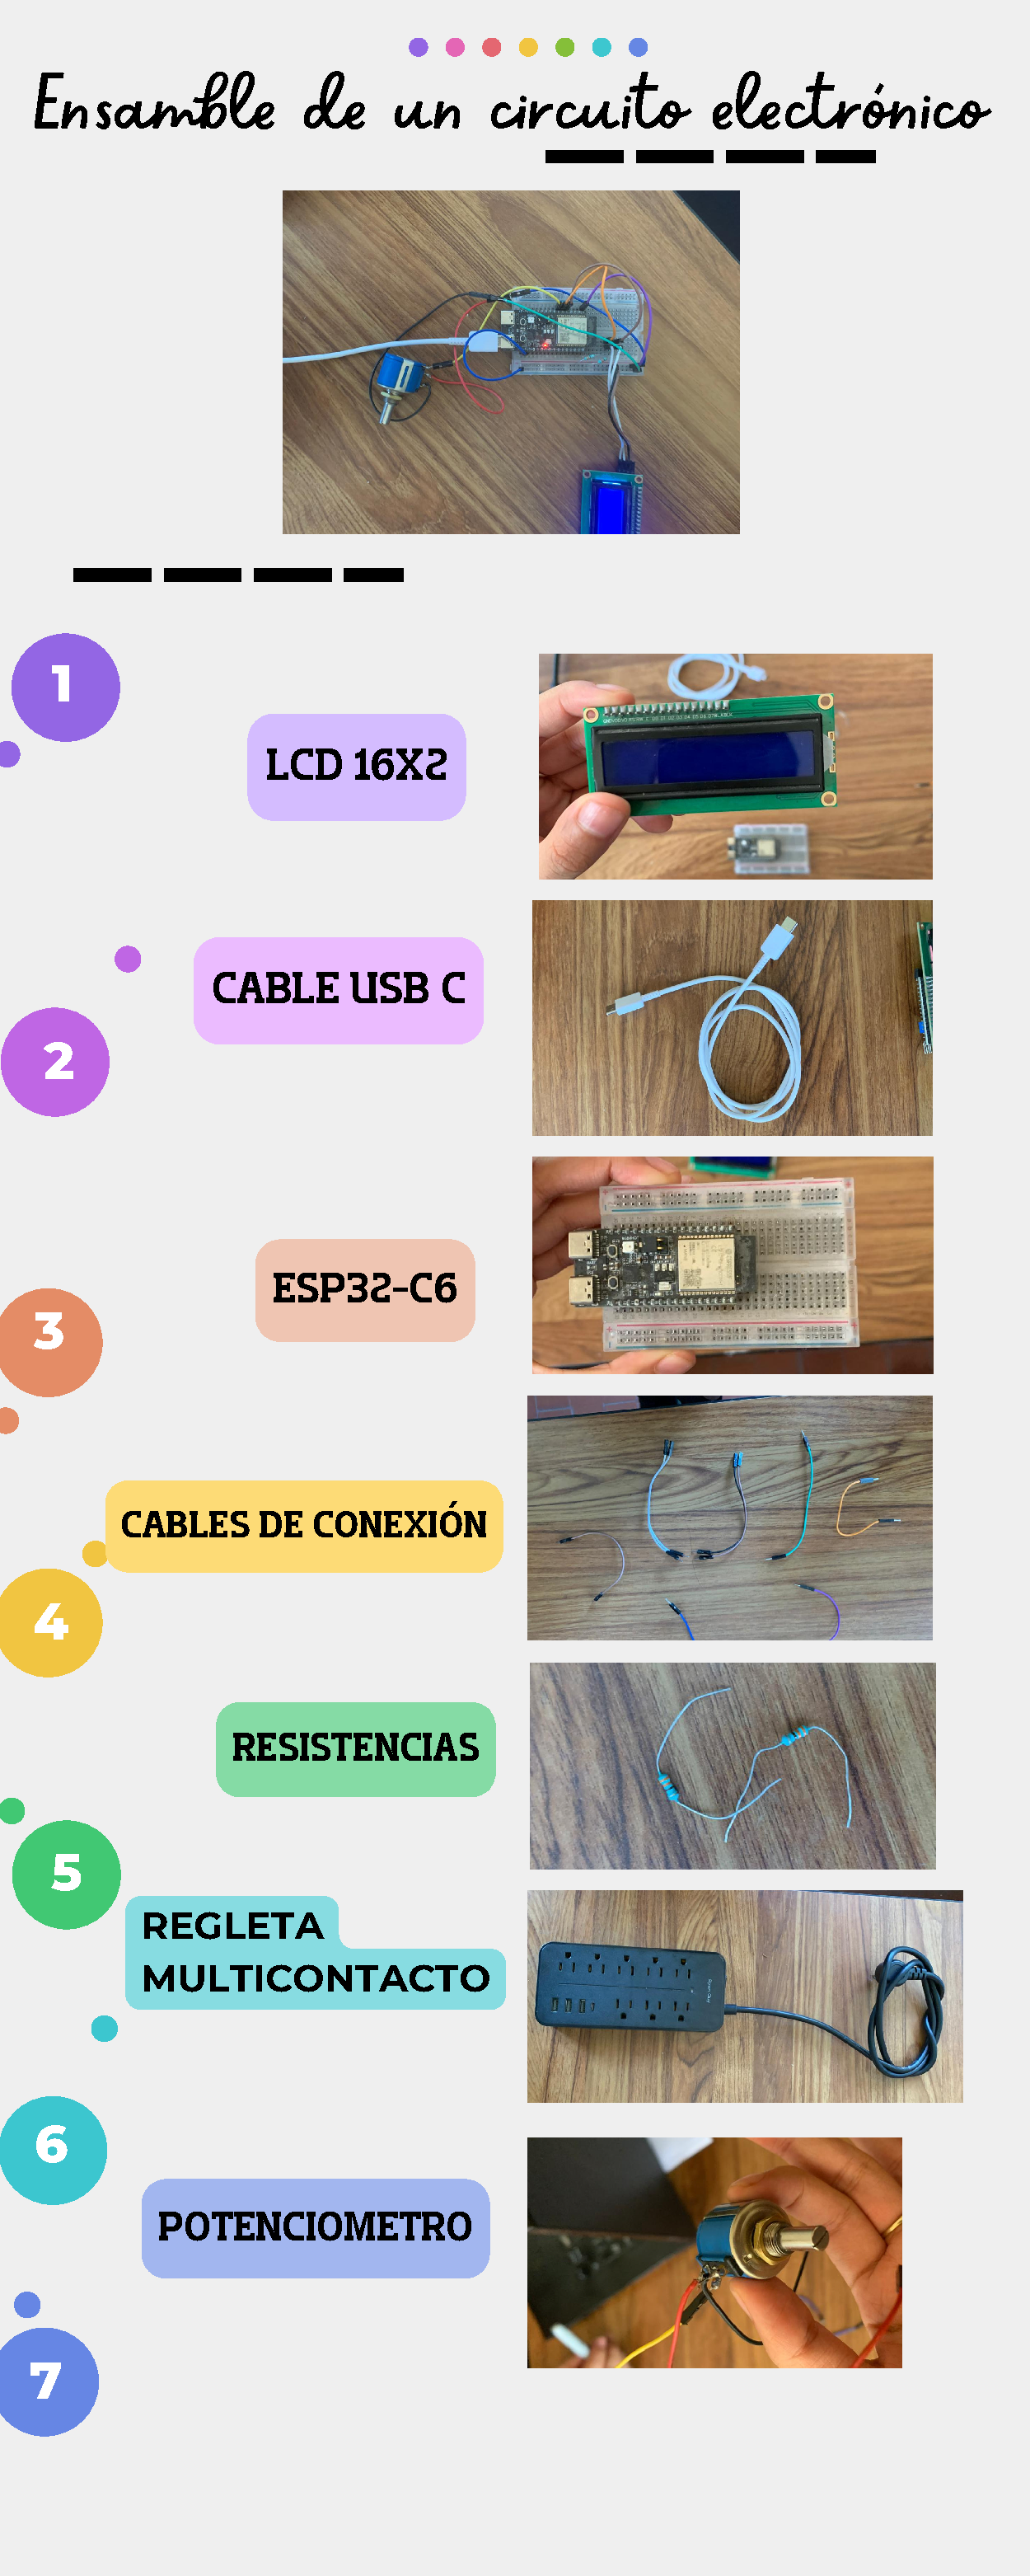
\includegraphics[trim = {25mm 50mm 20mm 140mm},clip,scale=0.5]{16/Img/Materiales C.E .pdf}
        \caption{Materiales}
        \label{fig:Materiales}
    \end{figure}
    % 
    % 
    % 
    % 
    \begin{figure}[H]
        \centering
        \includegraphics[trim = {10mm 10mm 10mm 10mm},clip,scale=0.150]{16/Img/Cables de conexión.PDF}
        \caption{Cables de conexión}
        \label{fig:Cables de conexión}
    \end{figure}
    % 
    % 
    % 
    % 
    \begin{figure}[H]
        \centering
        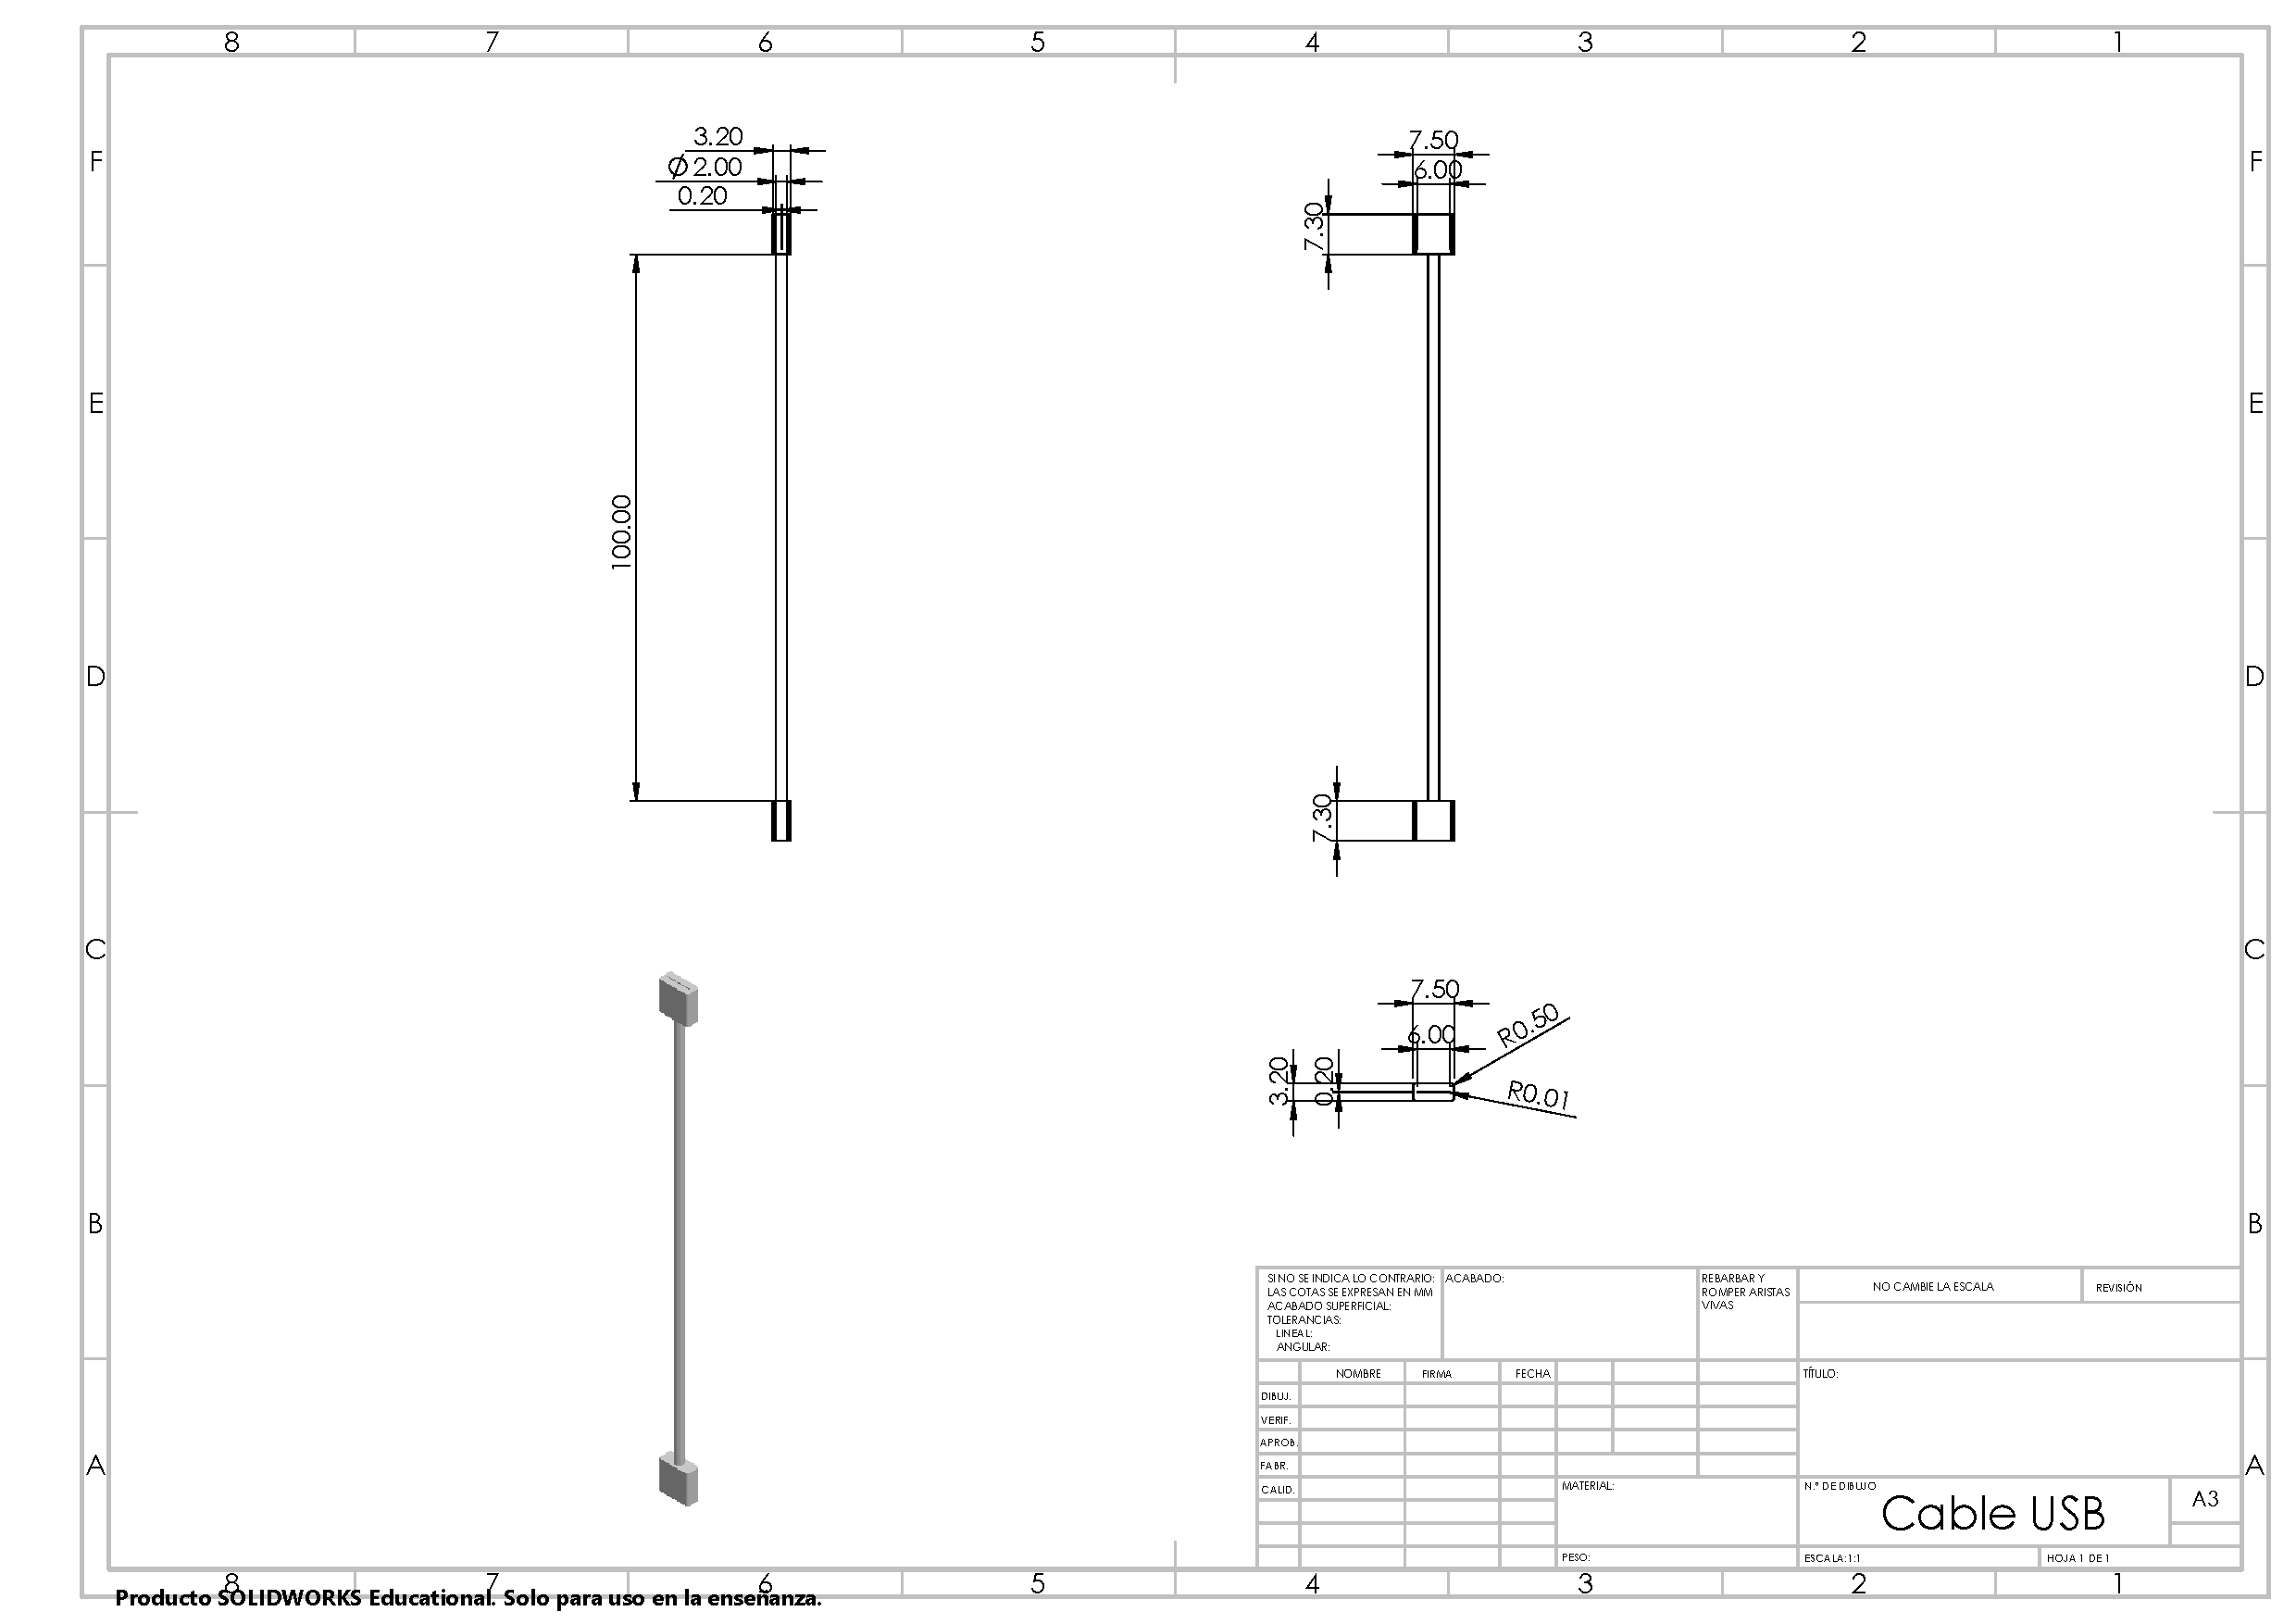
\includegraphics[trim = {10mm 10mm 10mm 10mm},clip,scale=0.150]{16/Img/Cable USB.PDF}
        \caption{Cables USB}
        \label{fig:Cable USB}
    \end{figure}
    % 
    % 
    % 
    % 
    \begin{figure}[H]
        \centering
        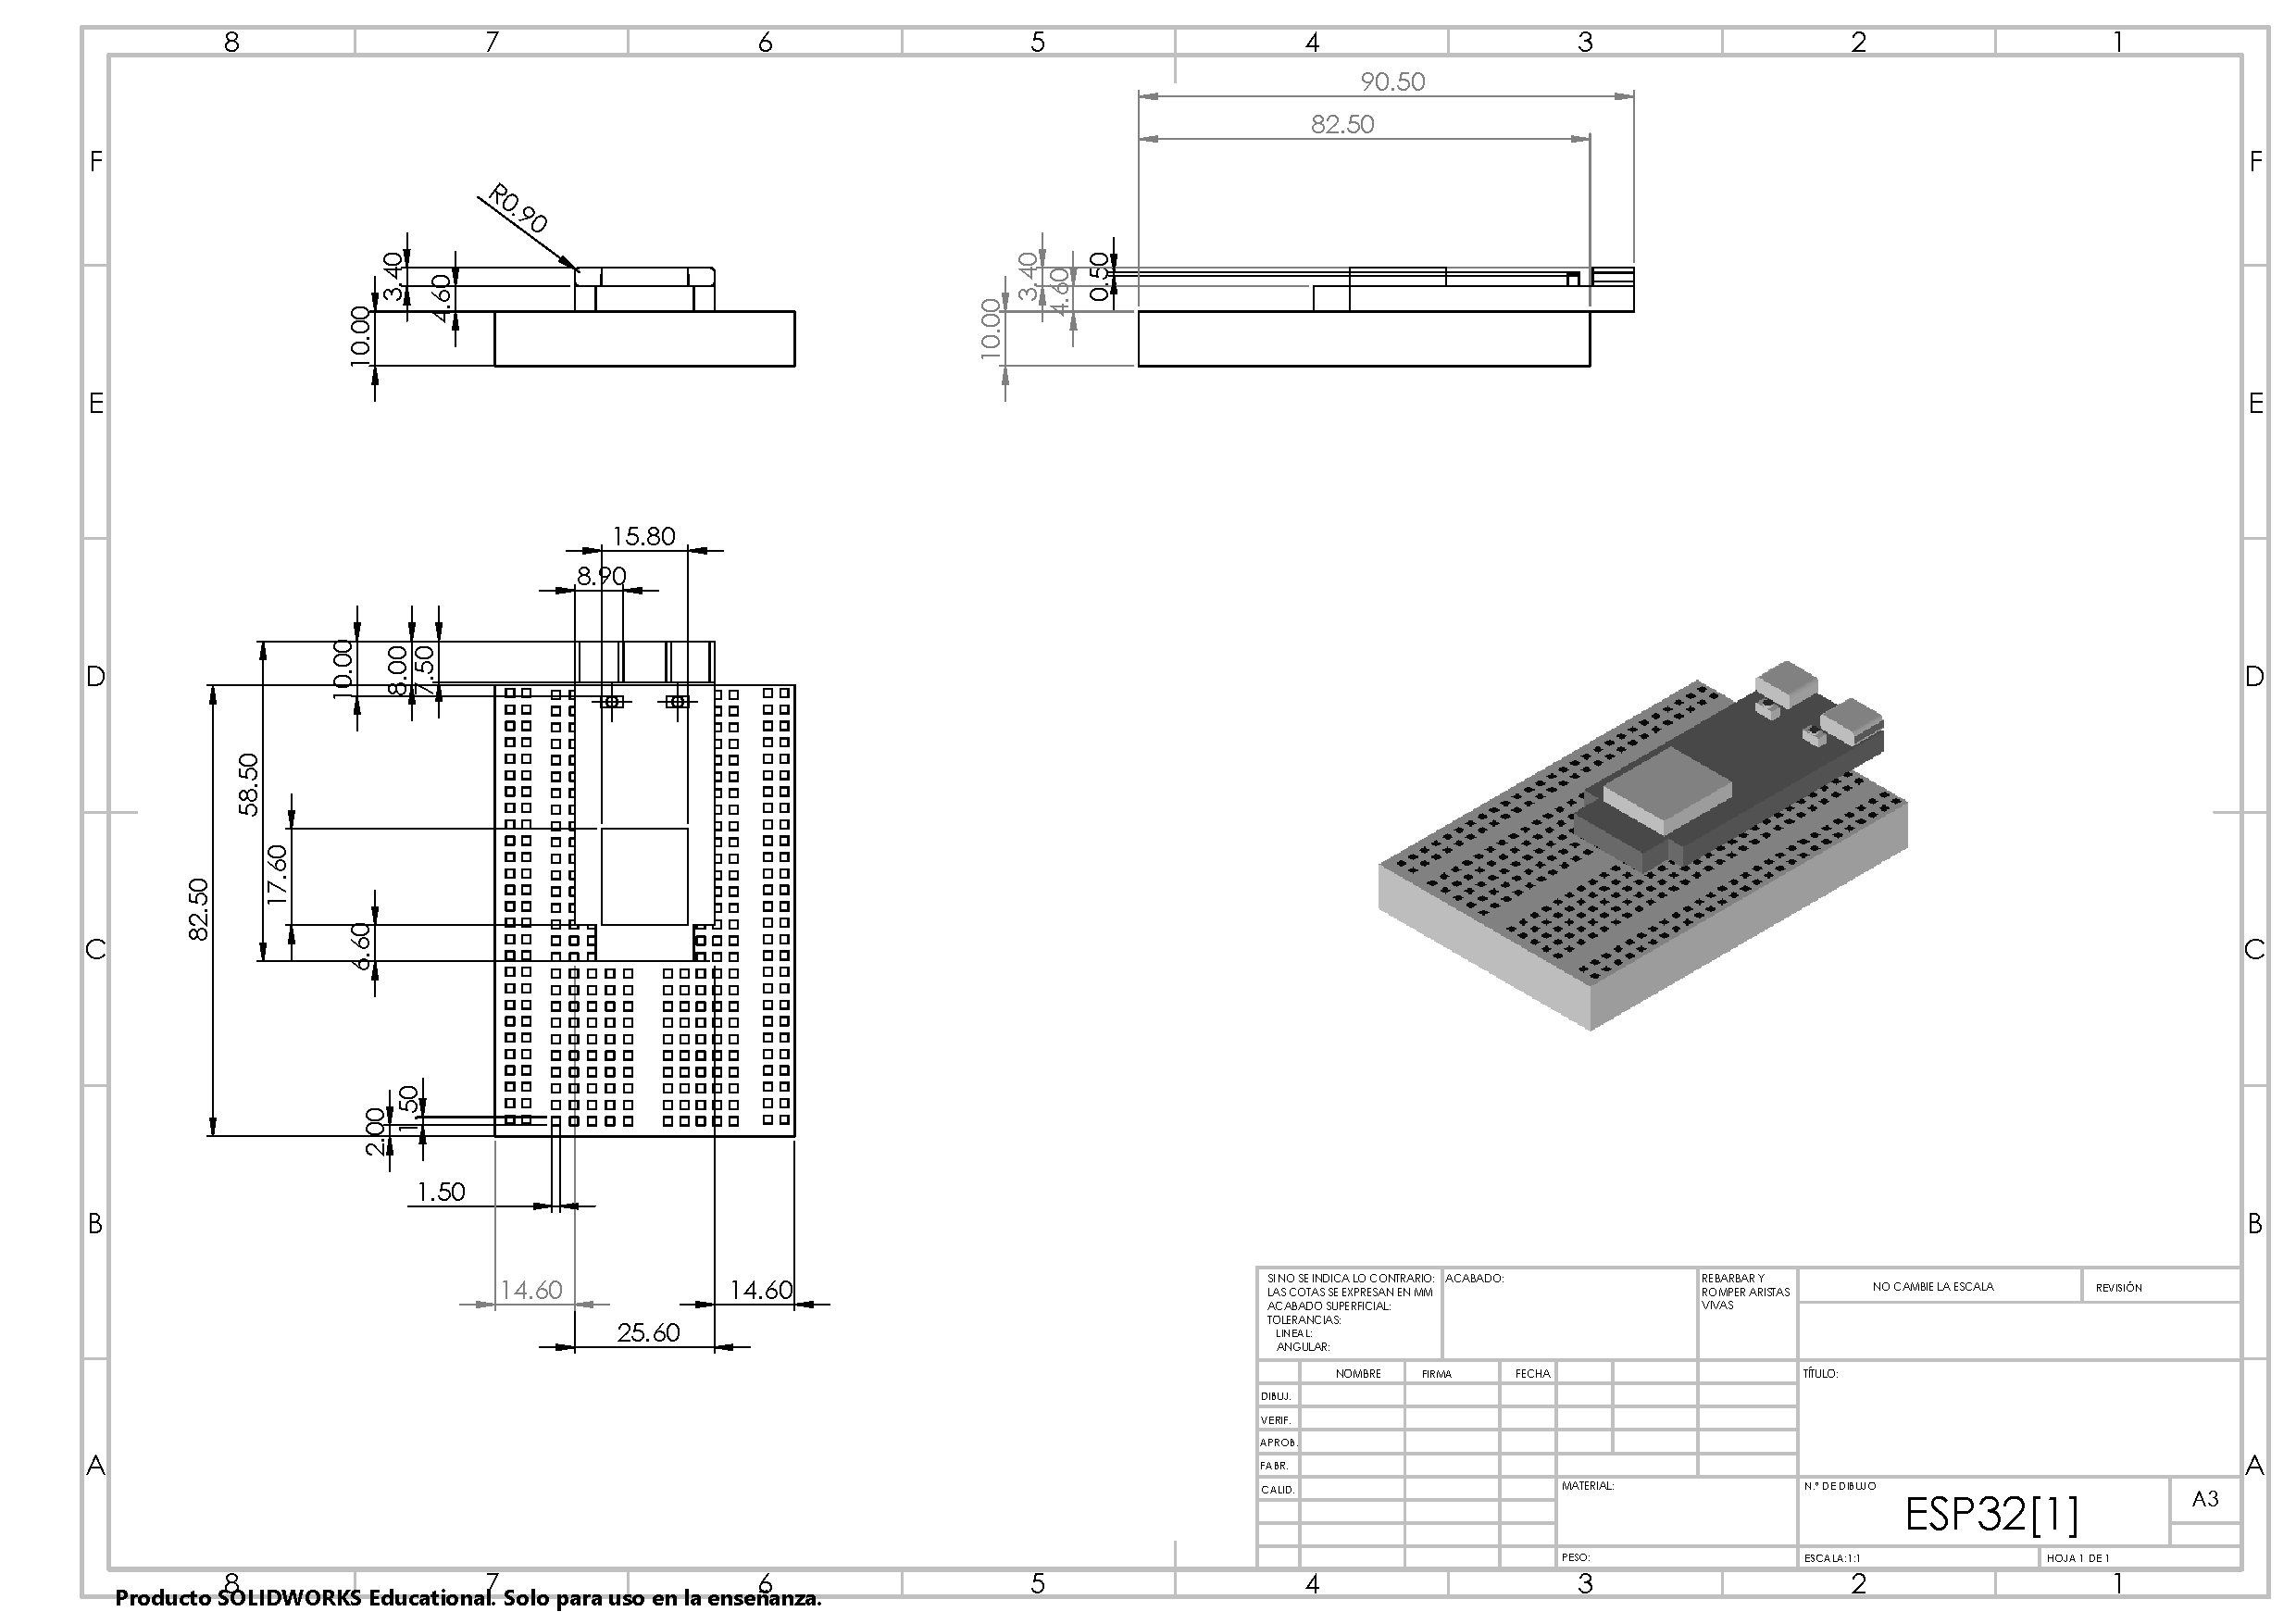
\includegraphics[trim = {10mm 10mm 10mm 10mm},clip,scale=0.150]{16/Img/ESP32.PDF}
        \caption{ESP32-C6}
        \label{fig:ESP32-C6}
    \end{figure}
    % 
    % 
    % 
    % 
    \begin{figure}[H]
        \centering
        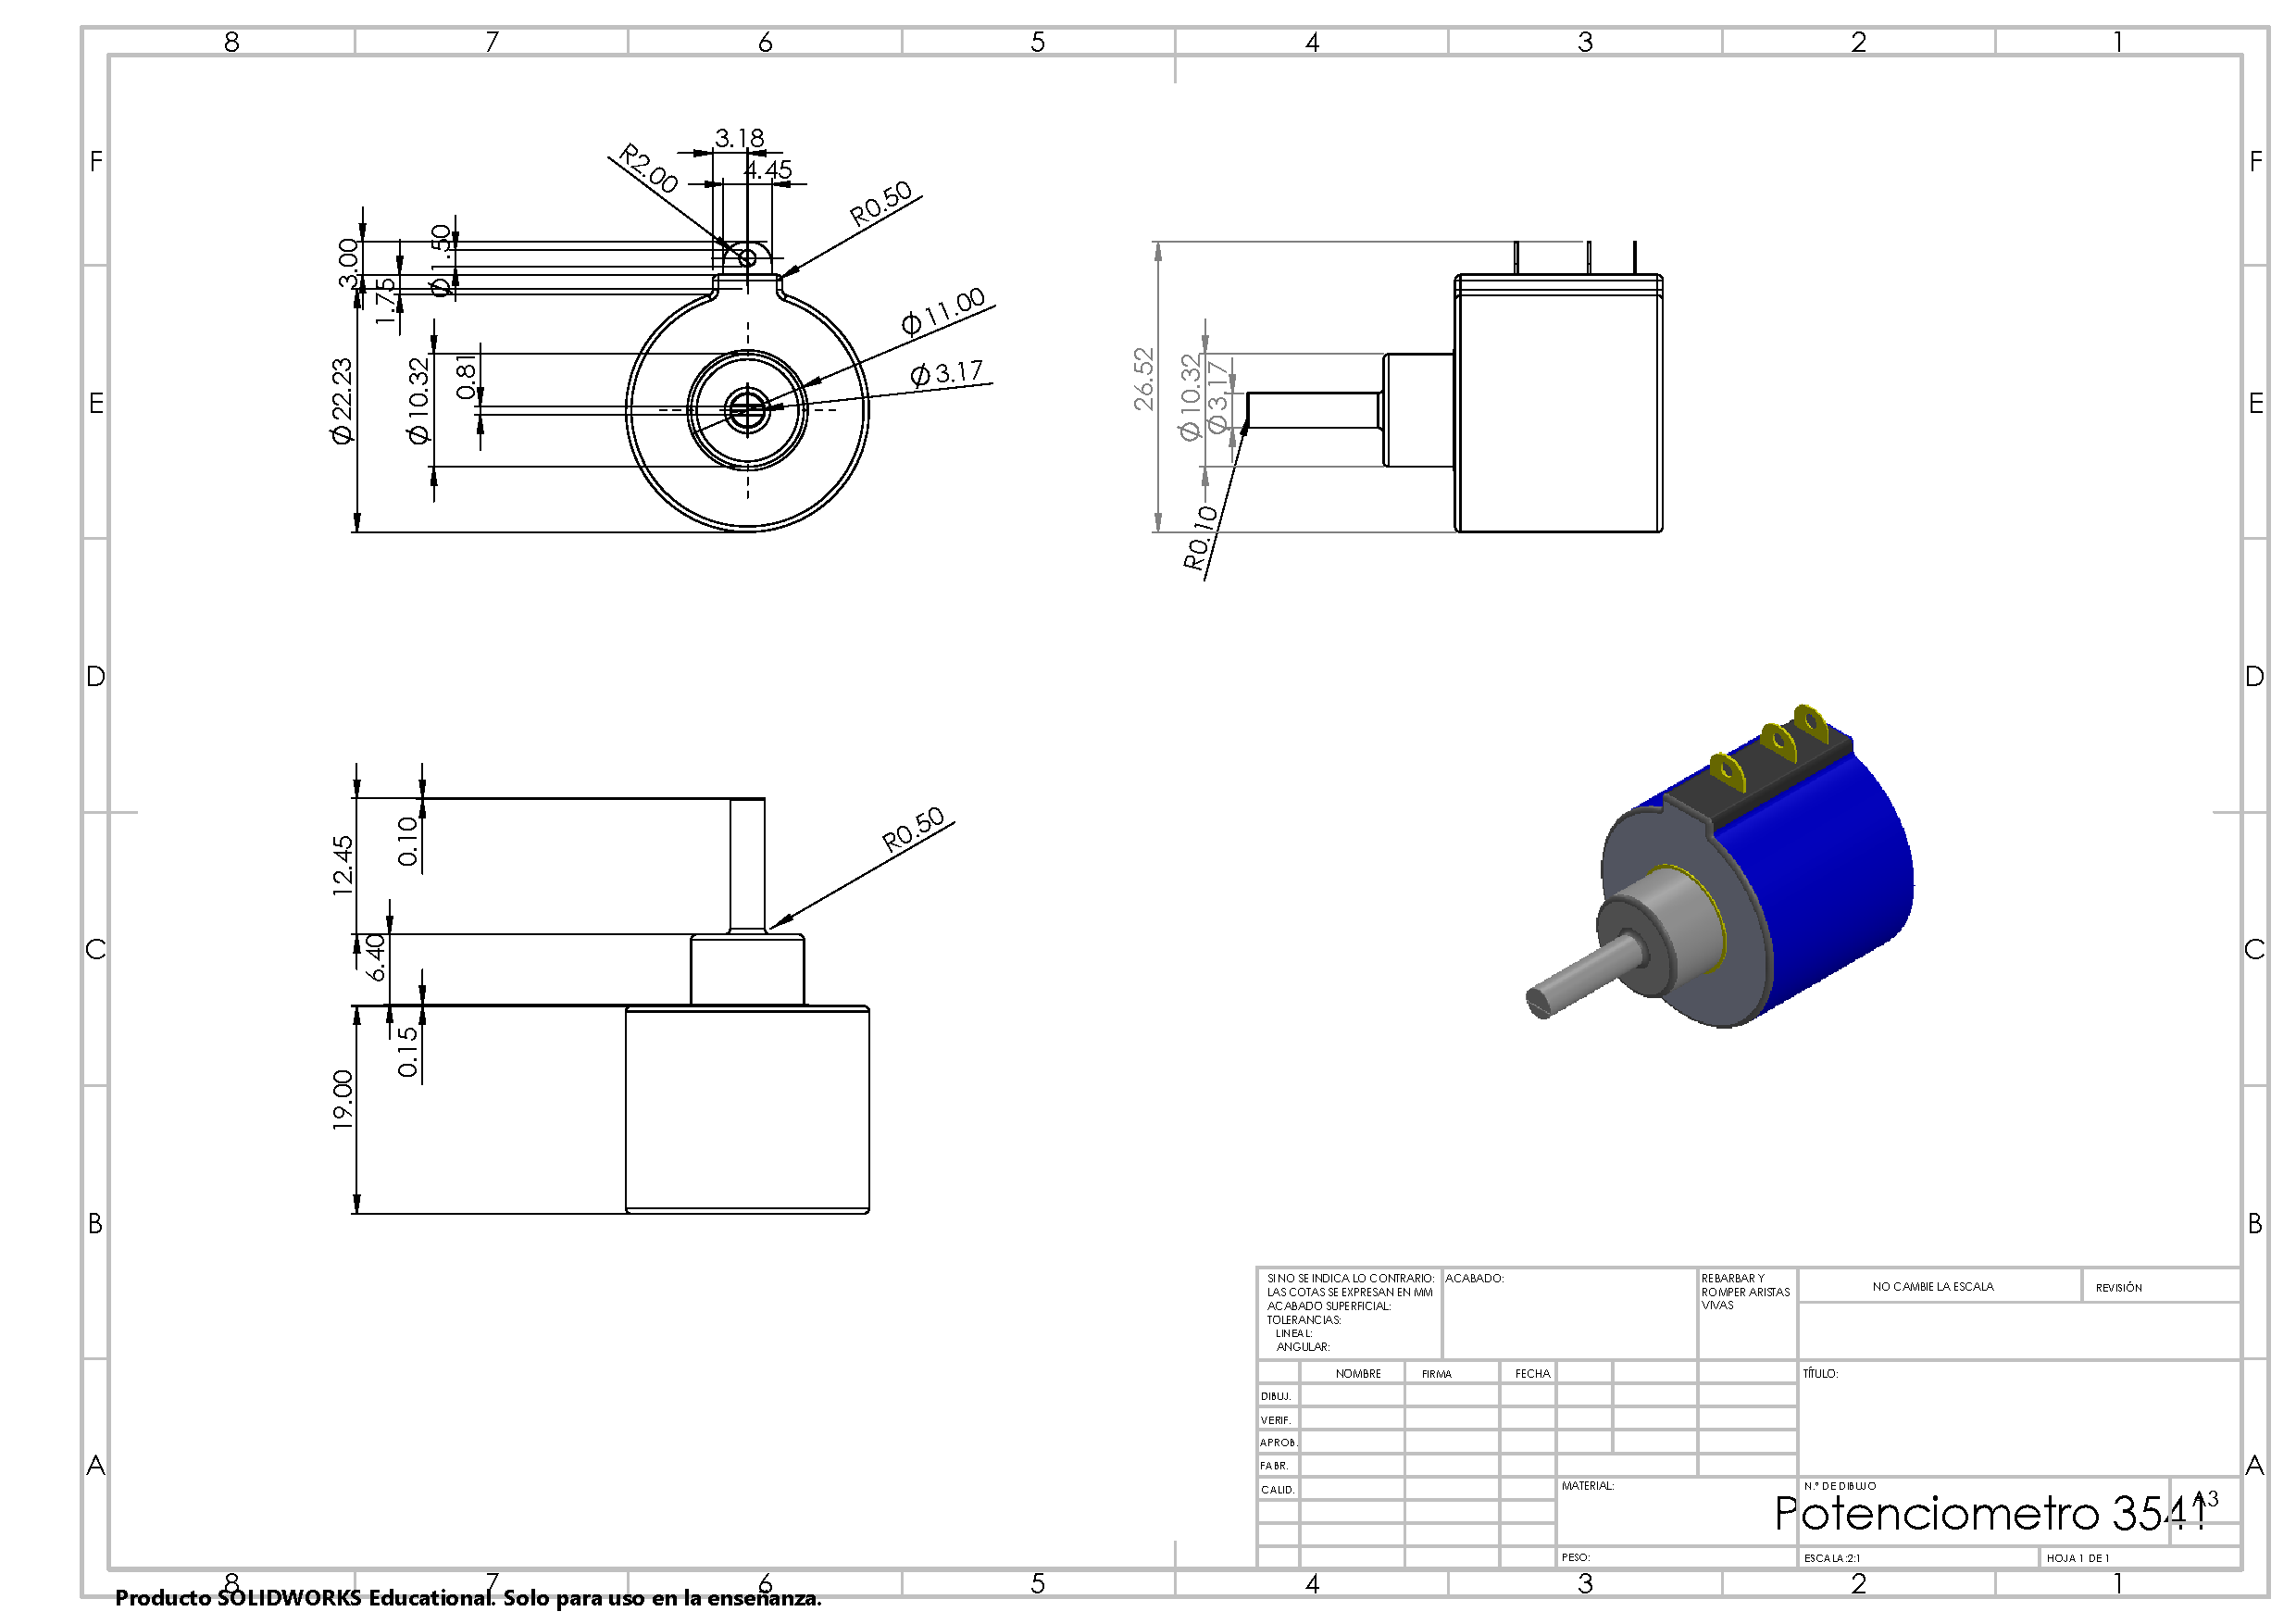
\includegraphics[trim = {10mm 10mm 10mm 10mm},clip,scale=0.150]{16/Img/Potenciometro 1KOH.PDF}
        \caption{Potenciometro}
        \label{fig:Potenciometro}
    \end{figure}
    % 
    % 
    % 
    % 
    \begin{figure}[H]
        \centering
        \includegraphics[trim = {10mm 10mm 10mm 10mm},clip,scale=0.150]{16/Img/Cables de conexión MM .PDF}
        \caption{Cable de conexión MM}
        \label{fig:Cable de conexión MM}
    \end{figure}
    % 
    % 
    % 
    % 
    \begin{figure}[H]
        \centering
        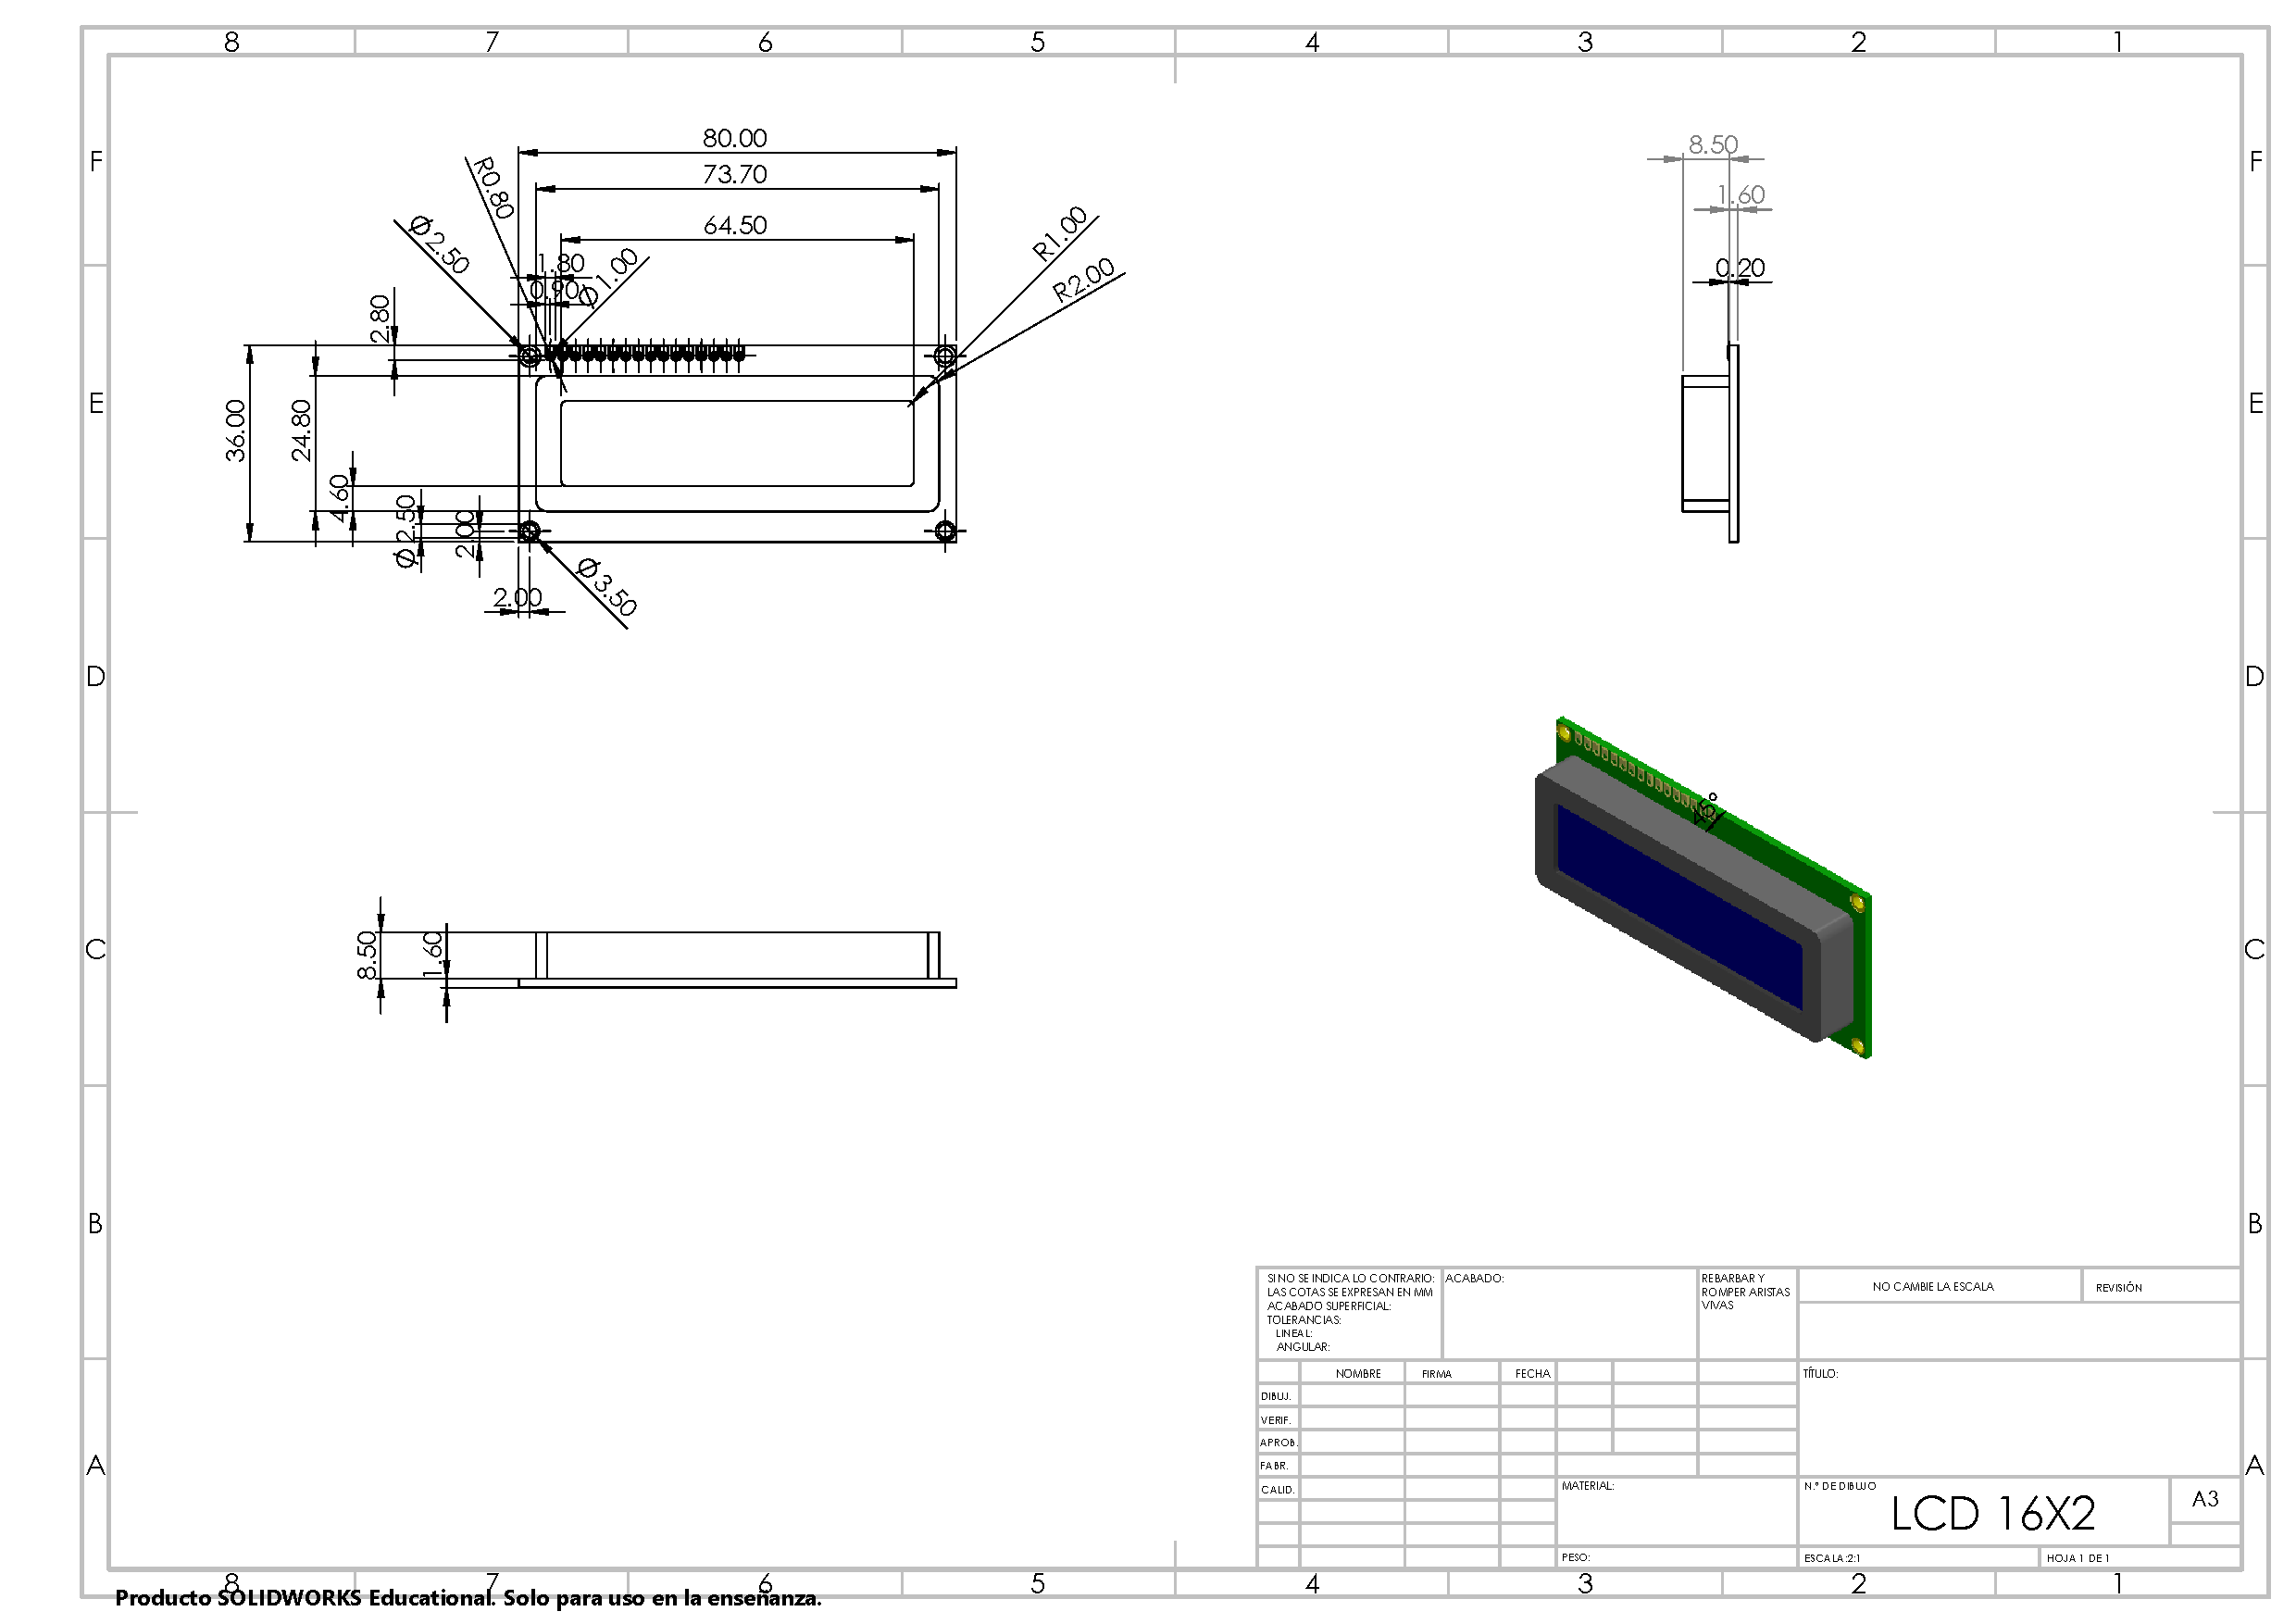
\includegraphics[trim = {10mm 10mm 10mm 10mm},clip,scale=0.150]{16/Img/LCD 16X2.PDF}
        \caption{LCD 16X2}
        \label{fig:LCD 16X2}
    \end{figure}
    % 
    % 
    % 
    % 
    \begin{figure}[H]
        \centering
        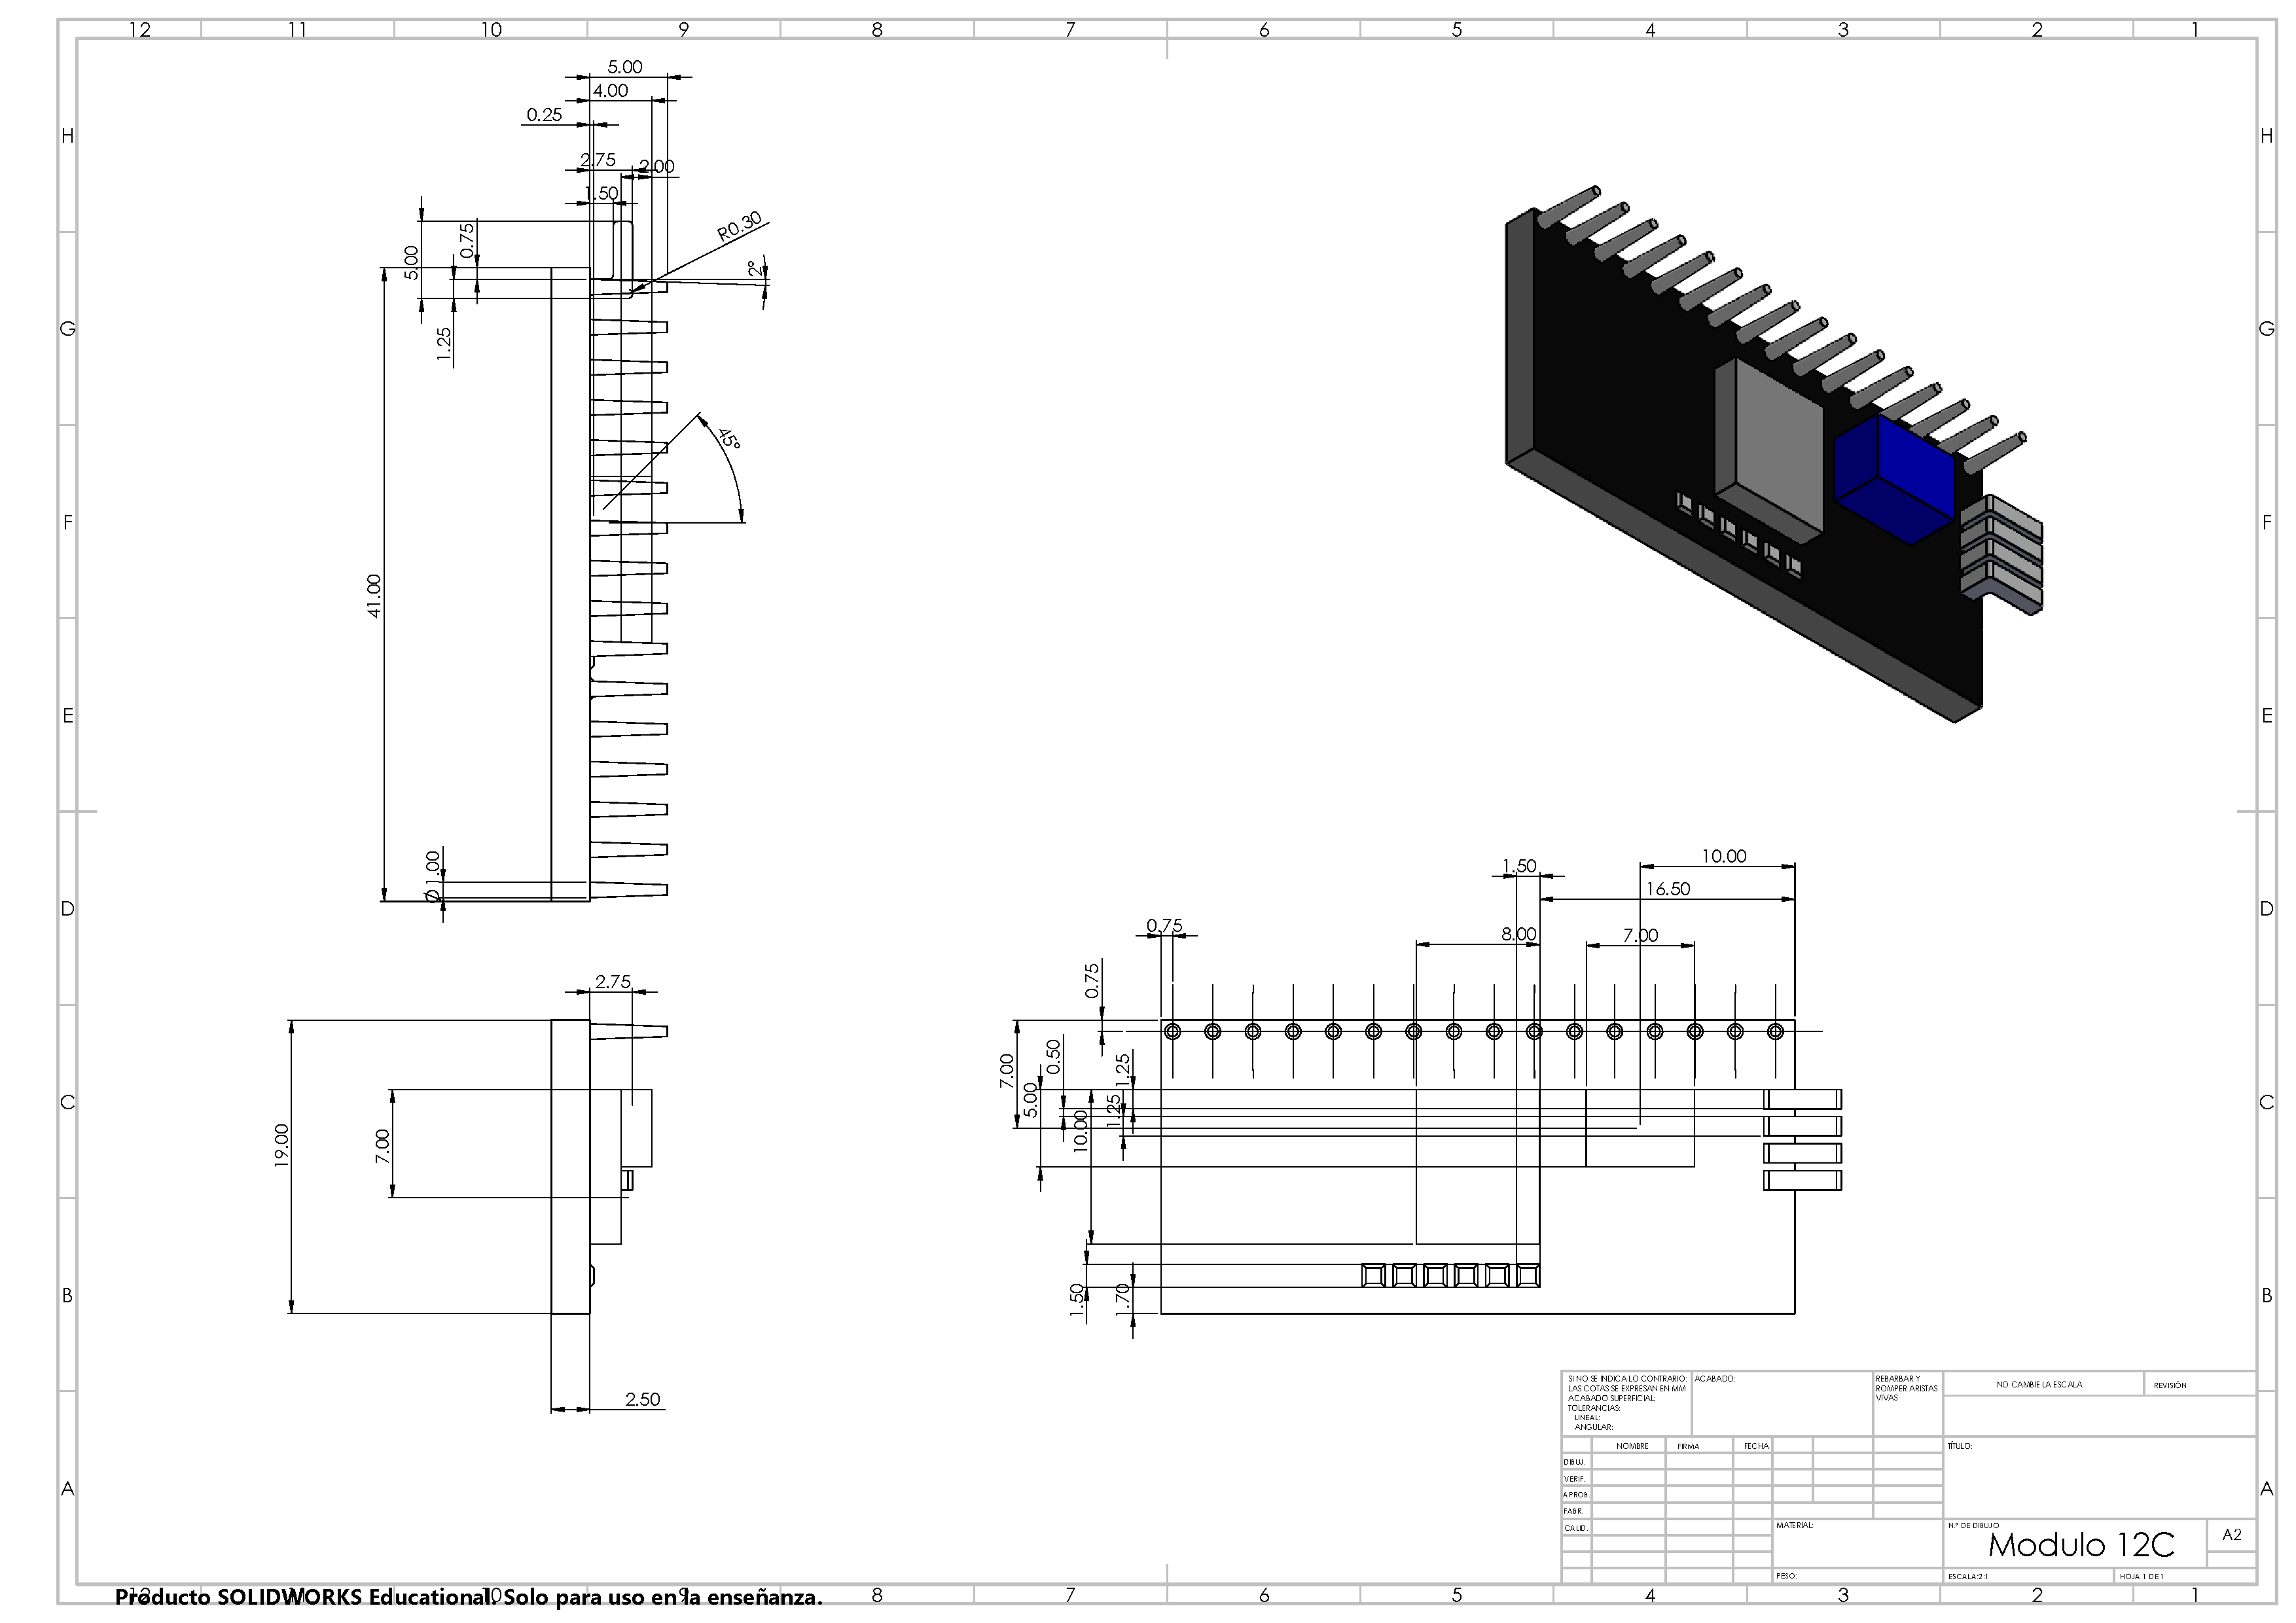
\includegraphics[trim = {10mm 10mm 10mm 10mm},clip,scale=0.150]{16/Img/Modulo 12C.PDF}
        \caption{Modulo 12C}
        \label{fig:Modulo 12C}
    \end{figure}
    % 
    % 
    % 
    % 
    \begin{figure}[H]
        \centering
        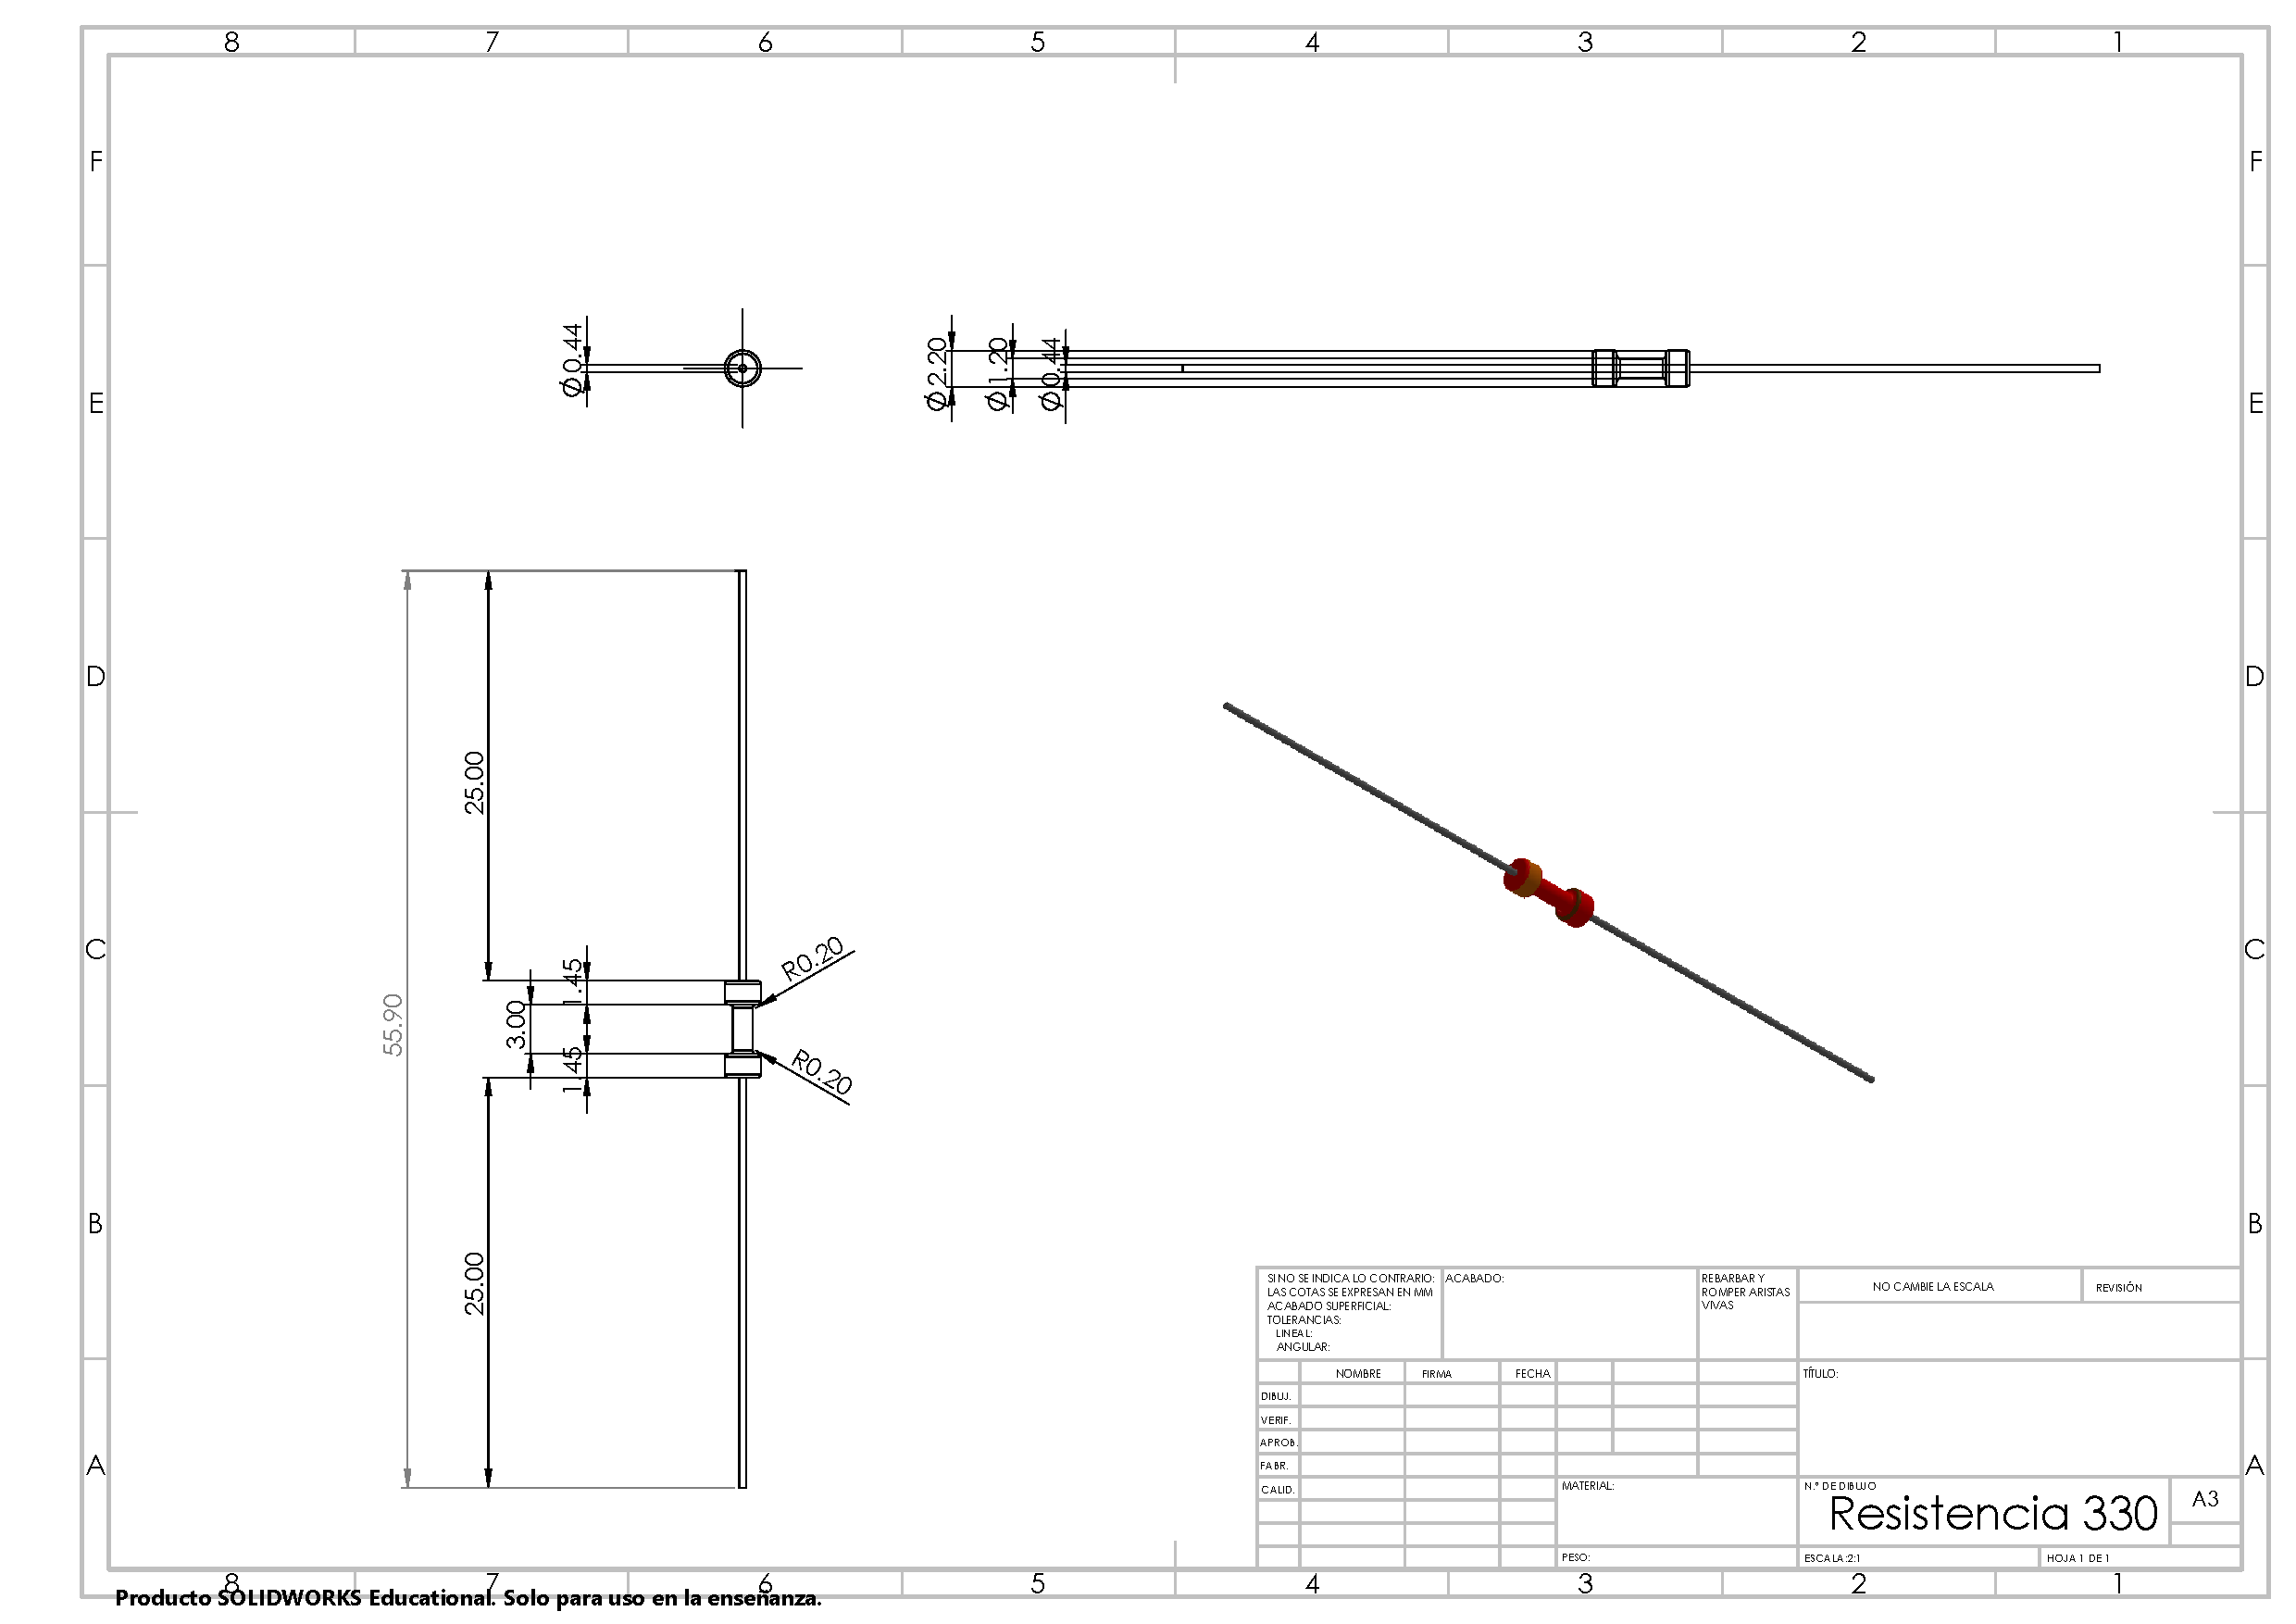
\includegraphics[trim = {10mm 10mm 10mm 10mm},clip,scale=0.150]{16/Img/Resistencia 330.PDF}
        \caption{Resistencia 330.PDF}
        \label{fig:Resistencia 330.PDF}
    \end{figure}
    % 
    % 
    % 
    % 
    \begin{figure}[H]
        \centering
        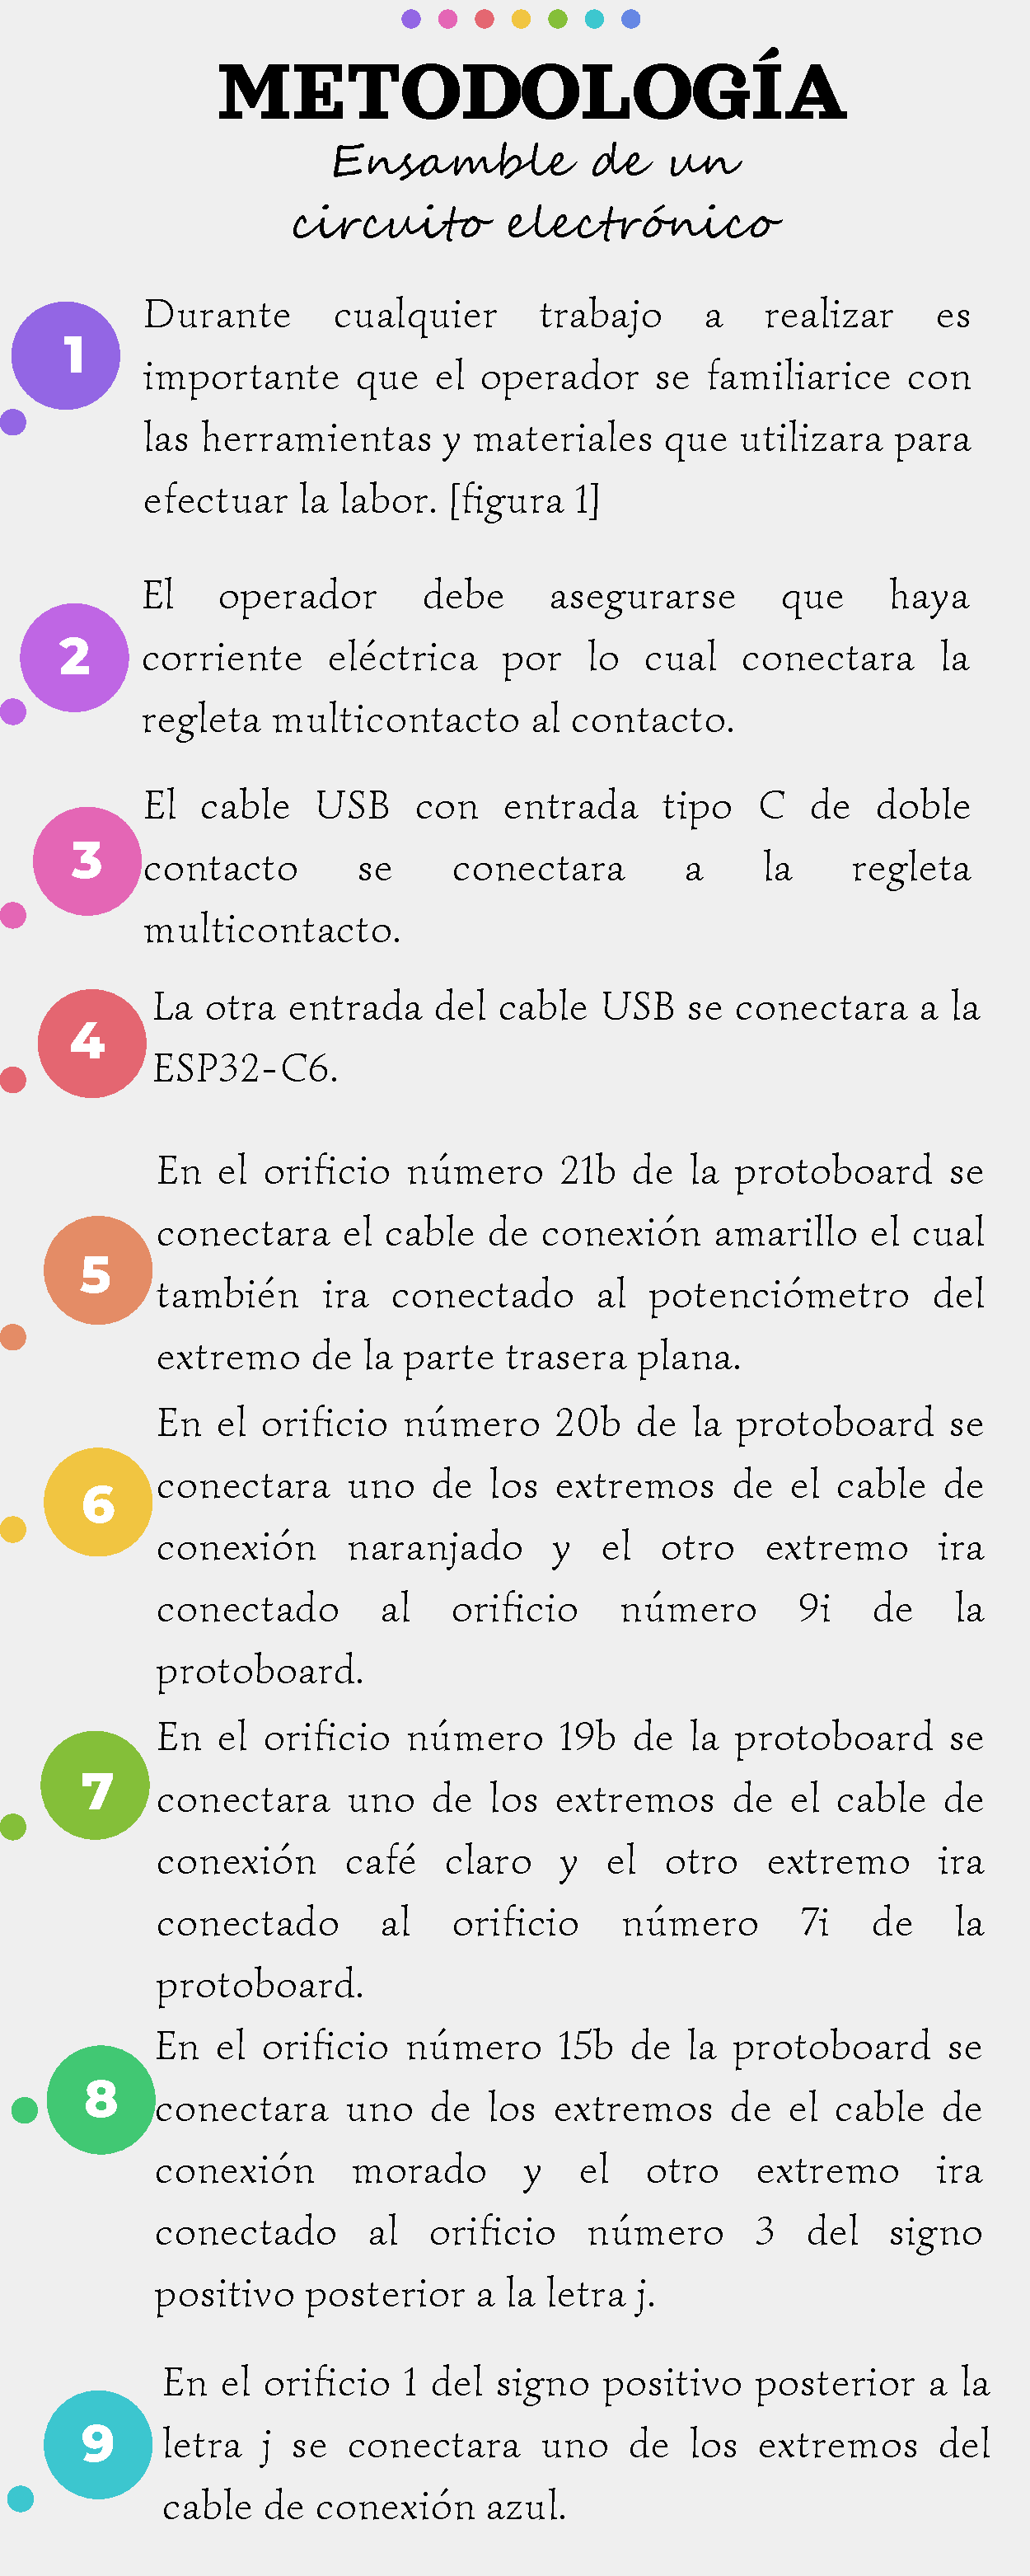
\includegraphics[trim = {5mm 10mm 5mm 50mm},clip,scale=0.4]{16/Img/Instructivo C.E (1).pdf}
        \caption{Metodología}
        \label{fig:metodología}
    \end{figure}
    % 
    % 
    % 
    % 
    \begin{figure}[H]
        \centering
        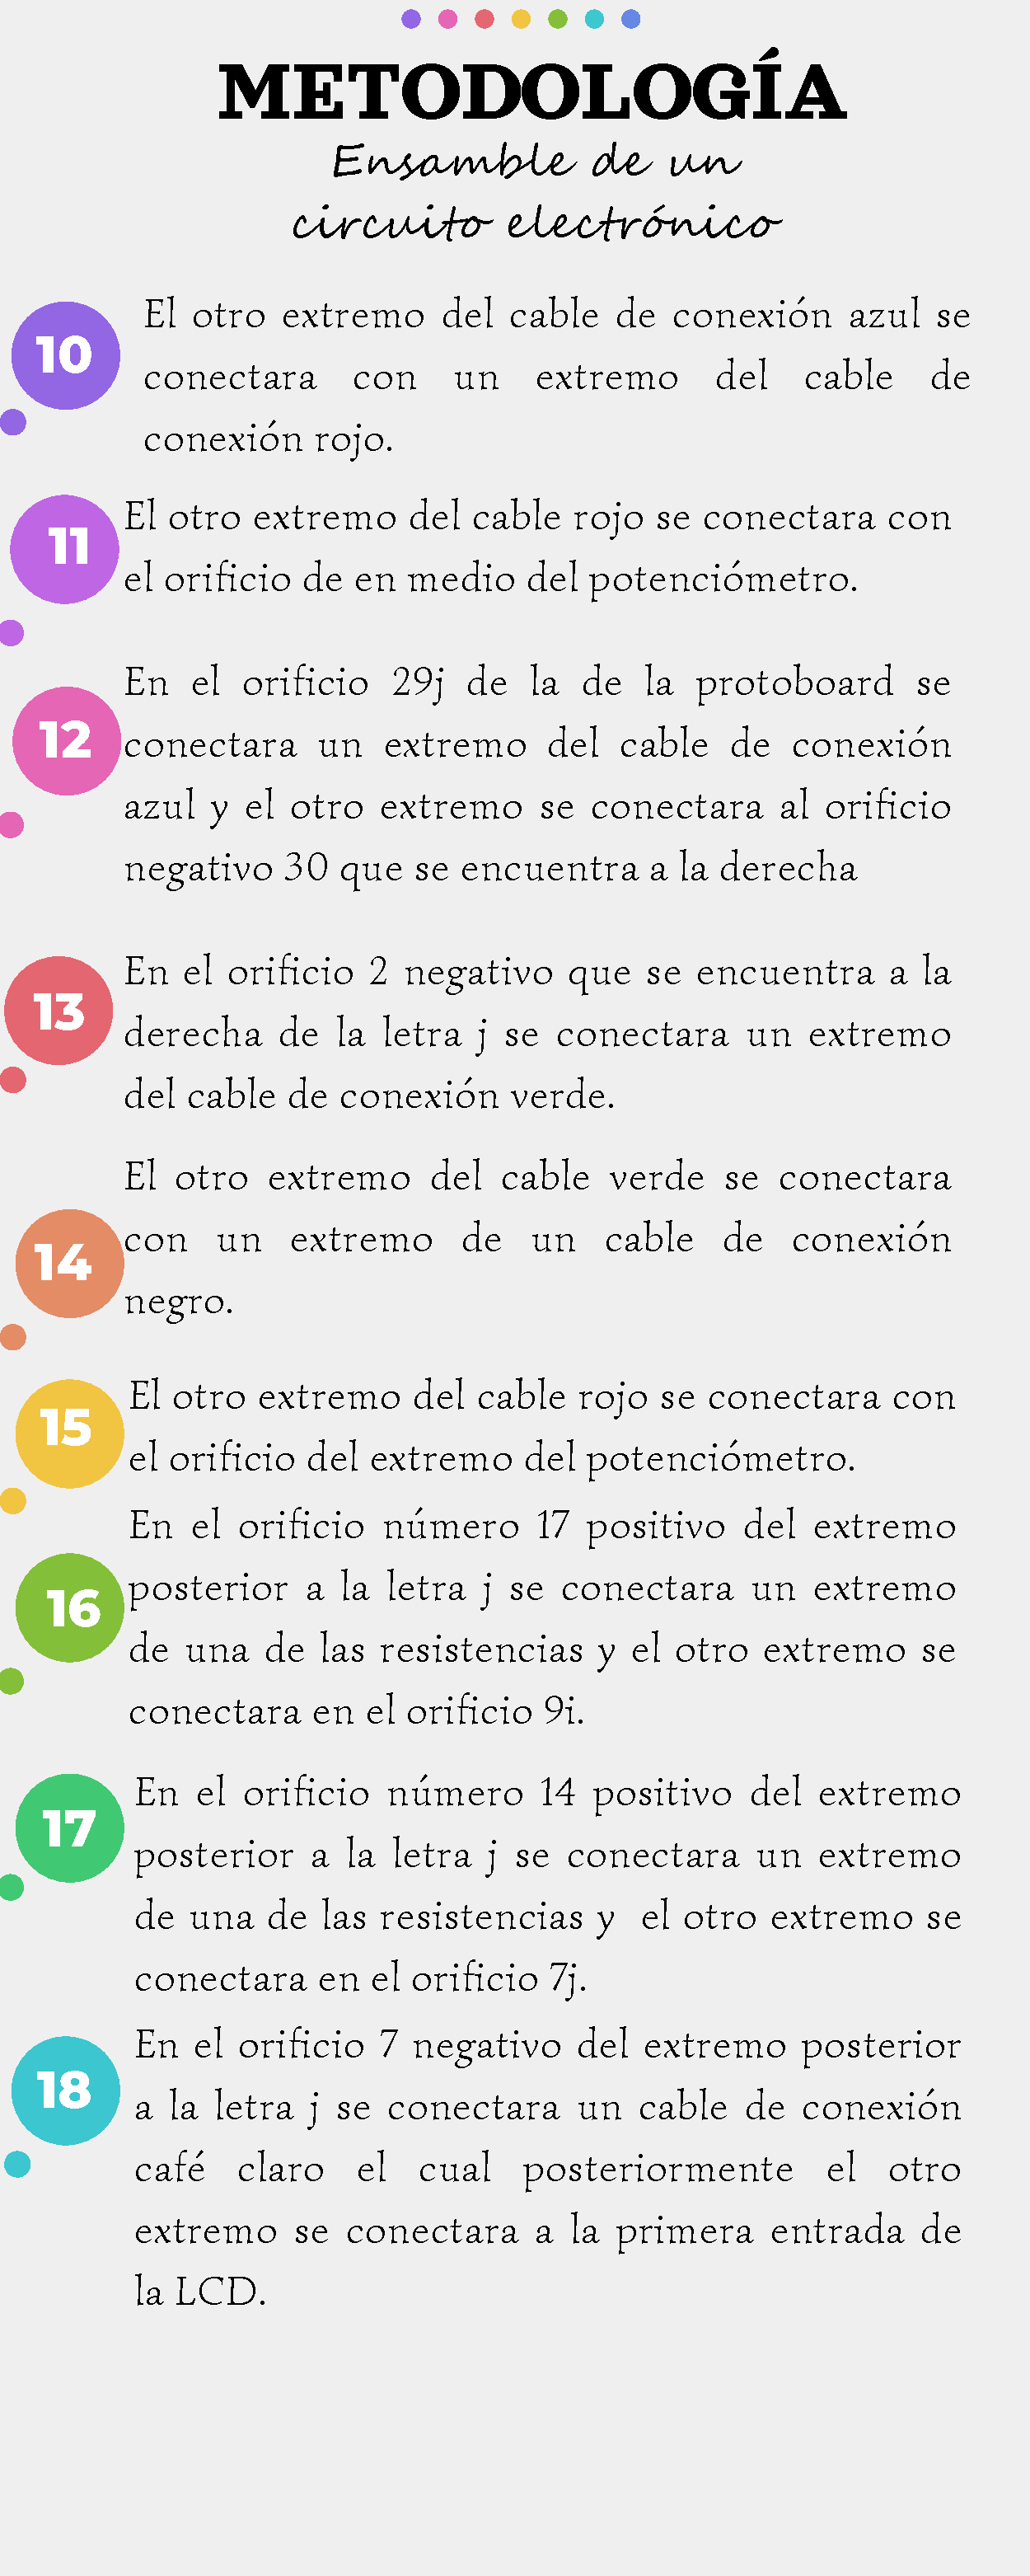
\includegraphics[trim = {5mm 10mm 5mm 50mm},clip,scale=0.4]{16/Img/Instructivo C.E (2).pdf}
        \caption{Metodología}
        \label{fig:metodología}
    \end{figure}
    % 
    % 
    % 
    % 
    \begin{figure}[H]
        \centering
        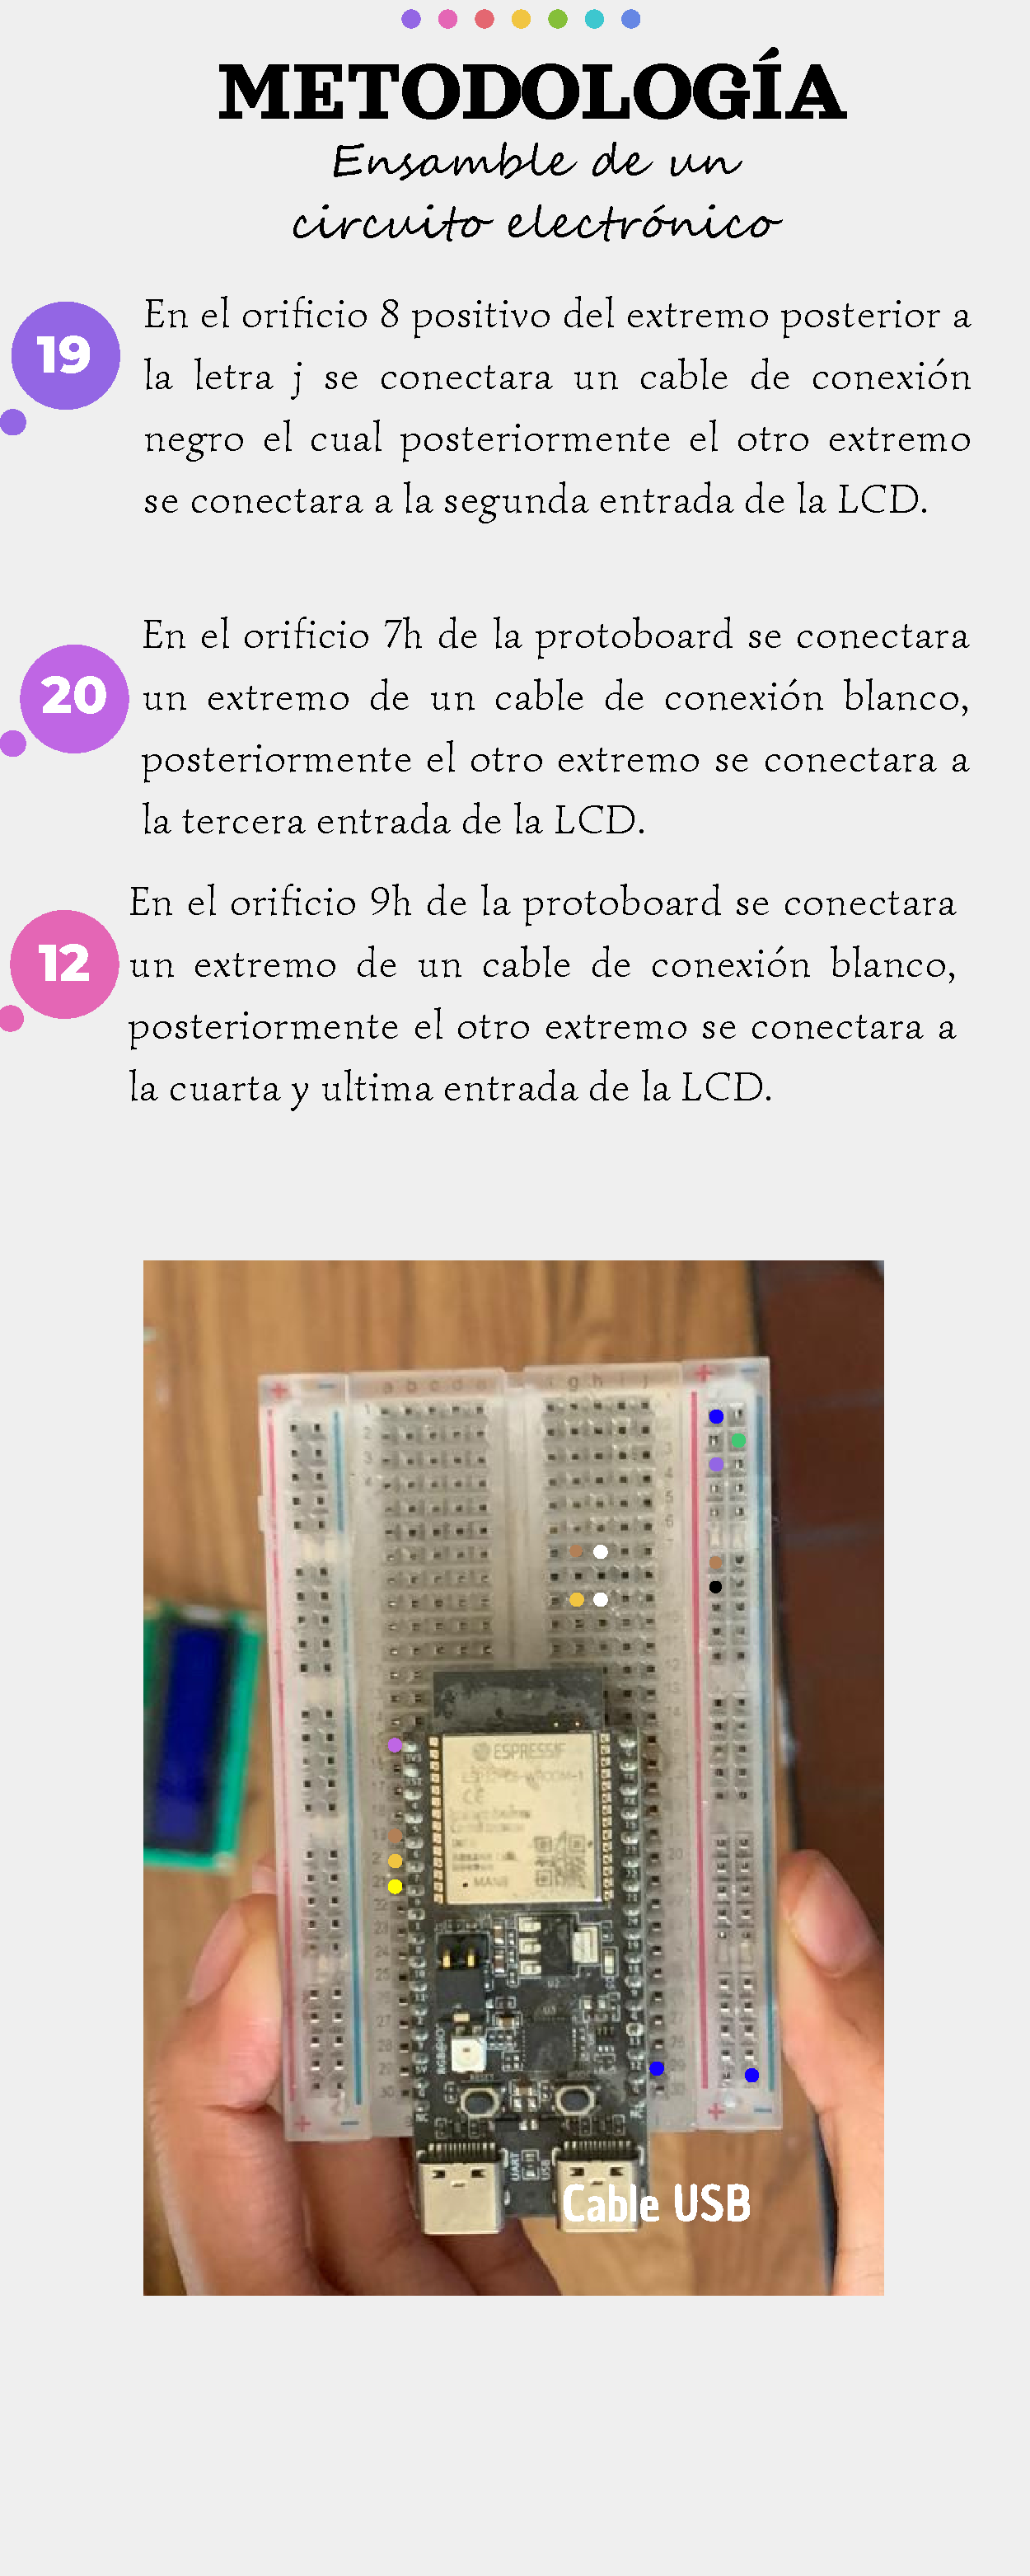
\includegraphics[trim = {5mm 10mm 5mm 50mm},clip,scale=0.4]{16/Img/Instructivo C.E (3).pdf}
        \caption{Metodología}
        \label{fig:metodología}
    \end{figure}
    % 
    % 
    % 
    % 
    \begin{figure}[H]
        \centering
        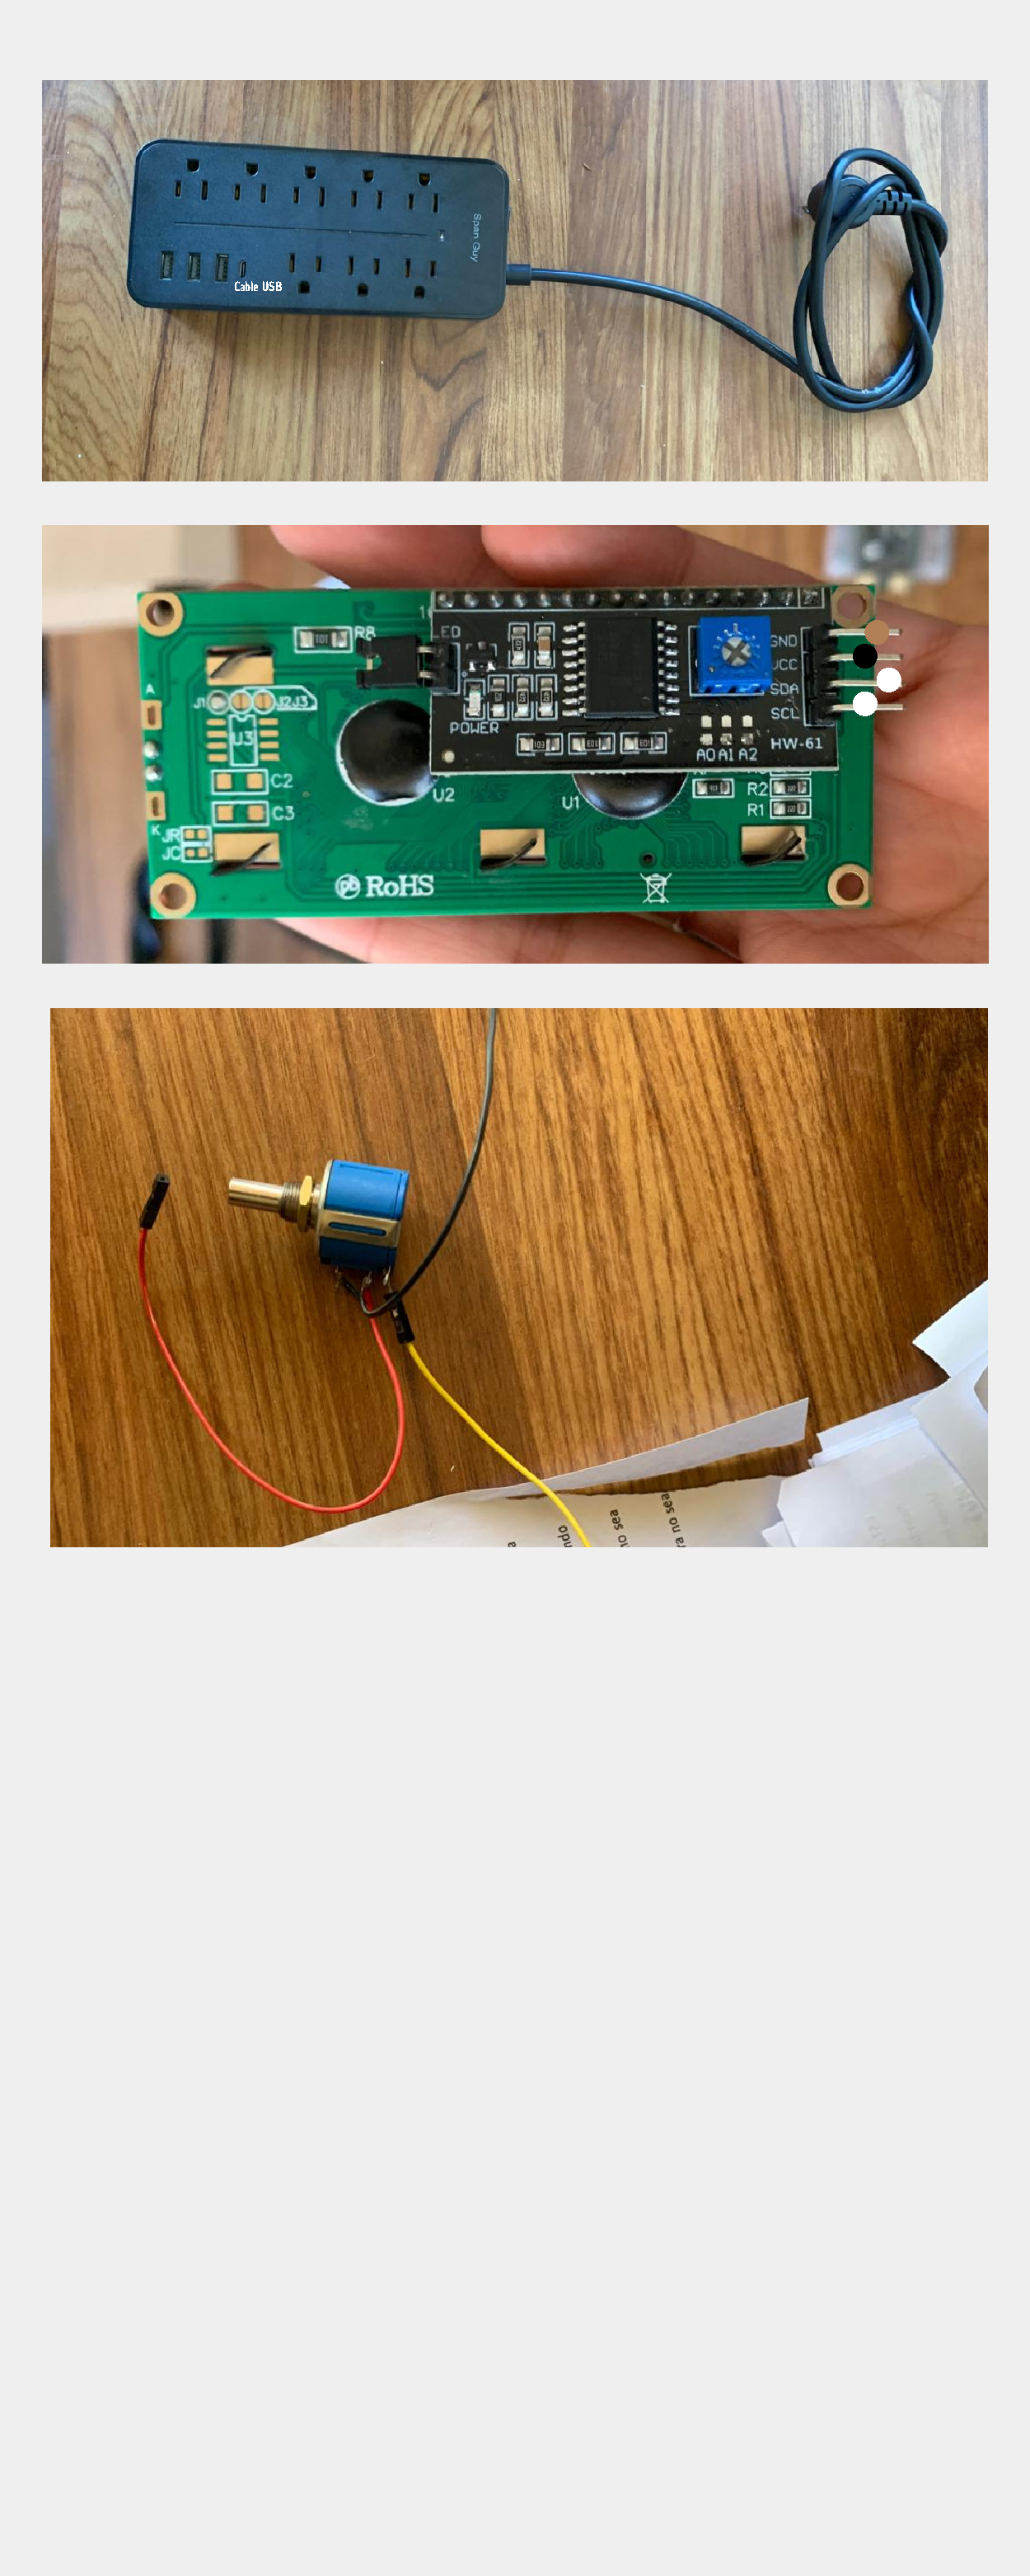
\includegraphics[trim = {5mm 180mm 5mm 30mm},clip,scale=0.4]{16/Img/Instructivo C.E (4).pdf}
        \caption{Metodología}
        \label{fig:metodología}
    \end{figure}
    % 
    % 
    % 
    Cada estrategia metodológica se establece acorde a cada objetivo, y por tanto deberá ser desglosada precisada y ordenada claramente. En consecuencia cada objetivo que se presentó en forma de verbo en infinitivo deberá determinar una estrategia en forma de adverbio. Ej. Desarrollar…Desarrollo. Son las actividades ordenadas que tienen como finalidad la prueba de la hipótesis. 
    
    \begin{itemize}
        \item Se debe establecer que se habrá de hacer, como, conque, y donde para obtener la información que permita probar la hipótesis.  
        \item Se debe desglosar de acuerdo a los objetivos específicos. 
        \item Se debe establecer una estrategia metodológica por cada objetivo específico. De manera simplista se podría decir que se cambia el verbo en infinitivo por su respectivo adverbio.
        \item En cada objetivo se debe describir que método, que materiales y que equipo se usará para conseguirlo.
        \item Se deben tener referencias Figura \ref{fig:lcd-16x2}.
    \end{itemize}
    % 
    % 
    \begin{figure}[H]
    
    \end{figure}
    
    % 
    \subsection{Prepara tu documento}
    
    Antes de que comiences a utilizar esta plantilla, es recomendable que prepare la información que contendrá en un archivo aparte. 
    Ten preparadas tus gráficas, así como también las tablas aparte, para que sea más fácil integrarlo. 
    Se recomienda fuertemente el uso de \textbf{formato Enhanced Metafile (.emf) para imágenes y gráficas} de resolución óptima. 
    Finalmente, completa y organiza el contenido antes de darle el formato de esta plantilla. 
    
    \subsection{Acrónimos y Abreviaciones}
    
    Los acrónimos y abreviaciones deberán ser definidos únicamente la primera vez que aparecen en el texto, esto para que el lector entienda lo que significan.
    
    \subsection{Ecuaciones}
    
    Las ecuaciones son una excepción a las especificaciones prescritas de esta plantilla. 
    Deberá determinar si su ecuación debe escribirse o no utilizando la fuente Adobe Devangari. 
    Para crear ecuaciones multinivel, puede ser necesario tratar la ecuación como un gráfico e insertarla en el texto después de aplicar el estilo de la platilla.
    Las ecuaciones serán enumeradas de manera consecutiva, y el número de ecuación, entre paréntesis, se colocan al ras de la derecha, utilizando una tabulación derecha. 
    
    \begin{equation}
        \label{eq1}
        x + y = z 
    \end{equation}
    
    Es importante asegurarse de que los símbolos de la ecuación sean definidos antes o inmediatamente después de la ecuación. Utilice “(1)”, en vez de “Eq. 1” al enumerar las ecuaciones, excepto al principio de una oración: “La ecuación (\ref{eq1}) es…”
    
    \section{Resultados y discusión}
    
    Antes de comenzar a preparar tu artículo, es importante que lea primero la guía del autor, la cual incluye los temas o apartados que son necesarios para tener tu trabajo completo.
    Una vez completada la edición del texto, el documento está listo para el uso de esta plantilla. En este archivo recién creado, resalte todo el contenido e importe el archivo de texto preparado. Ahora esta listo para estilizar su documento.
    En esta sección se deben presentar todo lo obtenido de la sección 2, incluidas deducciones o efectos del desarrollo. También se podrán incluir subsecciones numeradas de la siguiente forma:
    
    \subsection{Autores y Afiliaciones}
    
    Para distinguir las afiliaciones de los autores, utilice superíndices iniciando con el número 1, 2, etc., sucesivamente, esto dependerá de la cantidad de los departamentos a los que estén afiliados los autores. En caso de que todos los autores pertenezcan a una mismo departamento e institución, utilizar sólo el superíndice 1. 
    
    \subsection{Identificar los encabezados}
    
    Se les recuerda a los autores que los encabezados deben de estar conforme los solicita la guía del autor. De ahí se puede adaptar el trabajo para que sea más fácil de entender para el lector.
    Los encabezados organizan los temas sobre una base relacional y jerárquica. Por ejemplo, el título del documento es encabezado del texto principal porque todo el material posterior se relaciona y elabora sobre este tema. 
    
    \subsection{Tablas y Figuras}
    
    \begin{enumerate}
        \item Posición de las tablas y figuras: Coloque las figuras y las tablas en la parte superior e inferior de las columnas. Evite colocarlos en medio. Las figuras y las tablas grandes pueden abarcar ambas columnas. Los títulos de las figuras deben de estar debajo de las mismas; los títulos de las tablas deben aparecer encima de ellas. Insértese las figuras y los cuadros después de citarse en el texto. Utilice la abreviatura “Fig. 1”, incluso al principio de una oración. 
    \end{enumerate}
    
    \section{Conclusiones}
    
    Se describe aquí el alcance del trabajo, logros obtenidos y perspectivas para el futuro de este. Se sugiere colocar información cuantitativa obtenida.
    
    \section{Agradecimientos}
    
    Es importante darles su debido reconocimiento a los laboratorios, instituciones, organizaciones, entre otros que han sido participes para la culminación de este trabajo. También es importante mencionar, fondos, proyectos, becas, entre otros que se le han otorgado al o los autores para realizar el trabajo de investigación. Ejemplo: “Los autores agradecen al Concejo Nacional de Ciencia y Tecnología por los recursos otorgados…”
    
    \section*{Referencias}
    
    
    
    %
    \item @book{book,
      author    = {Groover, M. P}, 
      title     = {Groover, M. P. (1997). Fundamentos de manufactura moderna: materiales, procesos y sistemas.},
      publisher = {Pearson Educación},
      address   = {},
      year      = 1997,
    \item @book{book,
      author    = {}, 
      title     = { (1980). Introduccion al Estudio del trabajo},
      publisher = { Dirección general de George Kanawaty},
      address   = {},
      year      = 1980,
    }
    %
    \item @misc{RAE,
     author={RAE},
     title={REAL ACADEMIA española: Diccionario de la lengua española, consulta [14/04/2024]}, 
     year={2024},
     publisher={versión 23.3 en línea},
     howpublished={https://dle.rae.es/estudio},
     edition={23.ª ed.} 
    \item @misc{RAE,
     author={RAE},
     title={REAL ACADEMIA española: Diccionario de la lengua española, consulta [14/04/2024]}, 
     year={2024},
     publisher={versión 23.3 en línea},
     howpublished={https://dle.rae.es/tiempo},
     edition={23.ª ed.} 
    \item @misc{RAE,
     author={RAE},
     title={REAL ACADEMIA española: Diccionario de la lengua española, consulta [14/04/2024]}, 
     year={2024},
     publisher={versión 23.3 en línea},
     howpublished={https://dle.rae.es/movimiento},
     edition={23.ª ed.} 
    }
    %
    %
    
    \bibliographystyle{ieeetr}
    \bibliography{16/referencias}
    % 
    % 
    %%%%%%%%%%%%%%%%%%%%%%%%%%%%%%%%%%
    \appendix
    %%%%%%%%%%%%%%%%%%%%%%%%%%%%%%%%%%
    % 
    % 
    \centering{\section[\appendixautorefname{}]{APÉNDICE}}
    
    \label{anexo:pines}
    %%%%%%%%%%%%%%%%%%%%%%%%%%%%%%%%%%%%%%%